\documentclass[9pt,twoside,lineno]{pnas-new}
% \usepackage[dvipsnames]{xcolor}
% \usepackage{times}
\usepackage{amsmath,amsthm,amssymb,setspace,enumitem,epsfig,titlesec,verbatim,array,eurosym,multirow,enumitem}
% \usepackage[sort&compress,numbers]{natbib}
\usepackage{caption}
% \usepackage[margin=2.5cm, includefoot, footskip=30pt]{geometry}
% \usepackage{standalone}
% \usepackage{subcaption}
% \usepackage{hyperref}
% \usepackage{tabularx}
% \usepackage{booktabs}
% \usepackage{blkarray}
\usepackage[algo2e,ruled,vlined]{algorithm2e}
% \smallskip
% \renewcommand{\baselinestretch}{1.15}
% \usepackage{tikz}
% \usetikzlibrary{arrows}
% \usepackage{minitoc}
% \usepackage{graphicx}
% \usepackage{hyperref}
% \usepackage{subcaption}
% \usepackage{multirow}
% \usepackage{multicol}
% \usepackage{standalone}

\newtheoremstyle{plainCl1}% name
{12pt}%      Space above, empty = 'usual value'
{12pt}%      Space below
{\it}% 	   Body font
{}%         Indent amount (empty = no indent, \parindent = para indent)
{\bfseries}% Thm head font
{}%        Punctuation after thm head
{\newline}% Space after thm head: \newline = linebreak
{}%         Thm head spec

\theoremstyle{plainCl1}
\newtheorem{theorem}{Theorem}
\newtheorem{lemma}{Lemma}
\newtheorem{corollary}{Corollary}
\newtheorem{proposition}{Proposition}



\newtheoremstyle{plainCl2}% name
{12pt}%      Space above, empty = 'usual value'
{12pt}%      Space below
{}% 	   Body font
{}%         Indent amount (empty = no indent, \parindent = para indent)
{\bfseries}% Thm head font
{}%        Punctuation after thm head
{\newline}% Space after thm head: \newline = linebreak
{}%         Thm head spec

\theoremstyle{plainCl2}
\newtheorem*{definition}{Definition}
\newtheorem{remark}{Remark}


\def\wsls{\texttt{WSLS}}
\def\tft{\texttt{TFT}}
\def\gtft{\texttt{GTFT}}
\def\allc{\texttt{ALLC}}
\def\alld{\texttt{ALLD}}
\def\tftatft{\texttt{TFT-ATFT}}
\def\capri{\texttt{CAPRI}}
\def\aon{\texttt{AON$_k$}}
\def\cure{\texttt{CURE}}

\def\alt{\texttt{Alternator}}


\templatetype{pnassupportinginfo}

\title{Conditional cooperation with longer memory}
\author{Nikoleta E. Glynatsi, Ethan Akin, Martin A. Nowak, Christian Hilbe}
\correspondingauthor{Nikoleta E. Glynatsi.\\E-mail: glynatsi@evolbio.mpg.de}


\begin{document}

\maketitle

%% Adds the main heading for the SI text. Comment out this line if you do not have any supporting information text.
\SItext

This document provides further details on the previous literature, our methodology, our analytical
findings, and our evolutionary simulations.
Section~\ref{section:literature} gives an overview of the existing literature on direct reciprocity with longer memory. 
For several important articles, we summarize which key question they explore, and how our article further contributes to this strand of work. 
Section~\ref{section:model} summarizes the model. 
Here, we introduce all relevant strategy spaces, and we show how to compute long-term payoffs for strategies with more than one-round memory. 
Section~\ref{section:results} contains our key analytical results. 
Here, we define partner strategies, we present an algorithm that allows us to verify whether a given reactive-$n$ strategy is a partner, and we apply this algorithm to fully characterize the reactive-$n$ partner strategies for $n\!=\!2$ and $n\!=\!3$.
We perform a similar analysis for the stable defecting strategies. 
Finally, Section~\ref{section:simulations} presents some complementary evolutionary results. 
Finally, the Appendix in Section~\ref{section:appendix} contains the proofs of the mathematical results introduced in Section~\ref{section:results}. 



%%%%%%%%%%%%%%%%
%% LITERATURE REVIEW %%
%%%%%%%%%%%%%%%%

\section{An overview of the related literature}\label{section:literature}

By now, there is a vast literature on the evolution of reciprocal cooperation in repeated games. 
This literature has described various strategies that either succeed in evolutionary simulations and computer tournaments, or that exhibit some interesting theoretical properties. 
This literature also describes how results depend on parameters such as the benefit-to-cost of ratio, or the game's continuation probability. 
For a general overview on these results, we refer to the reviews and text books in Refs.~\cite{axelrod:book:1984,nowak:book:2006,sigmund2010,hilbe:Nature:2018,Glynatsi:HSSC:2021}. 
In the following we discuss some key papers that discuss the role of memory on direct reciprocity.

\subsubsection*{Particular higher-memory strategies}
First, there are several papers that highlight particular strategies with more than one-round memory. 
For example, Yi {\it et al} \cite{Do:JTB:2017} describes a variant of Tit-for-Tat (\tft), referred to as \tftatft. 
This strategy depends on the outcome of the last two rounds. 
It typically repeats the co-player's previous move; but in case the co-player defected because of an error, it chooses to do the opposite of the co-player's previous move.  
Compared to \tft, \tftatft{} is more robust with respect to implementation errors, and hence it emerges in some evolutionary simulations. 

Following up on this work, Baek and Murase \cite{murase:SciRep:2020} introduce a class of strategies called `friendly rivals'. 
These strategies establish mutual cooperation against themselves. 
At the same time, a player with such a strategy always gets at least the payoff of its opponent, irrespective of the opponent's strategy. 
In particular, such strategies satisfy our notion of being a partner. 
By explicitly considering all pure strategies with three rounds of memory, they identify one strategy that performs particularly well, referred to as \capri. 
In \cite{Murase:PLoSCompBio:2023a}, the authors examine whether friendly rivals emerge in an evolutionary setting. 
They conclude that friendly rivals play a minor role. 
Instead, partner strategies often seem to be sufficient to promote cooperation.

Hilbe et al~\citep{hilbe:PNAS:2017} use an axiomatic approach to derive stable memory-$n$ strategies of direct reciprocity. 
They impose three conditions on the strategies they look for: 
({\it i})~{\it Mutual cooperation:} Such a strategy ought to fully cooperate with itself. 
({\it ii})~{\it Retaliation:} Once a co-player defects, the strategy ought to defect for at least $k$ rounds. 
({\it iii})~{\it Error-correction:} When two players with that strategy interact, they return to mutual cooperation after at most $k$ rounds, after any possible previous history. 
The authors find that there is a class of memory-$n$ strategies that satisfies these properties. 
They refer to the elements of this class as All-or-None strategies, or~\aon. 
These \aon{} strategies satisfy the conditions for partner strategies. 
For $k\!=\!1$ they contain Win-Stay Lose-Shift~\cite{nowak:Nature:1993} as a special case. 

Finally, Li {\it et al} \cite{li:NatureCompSci:2022} describe a strategy of {\it cumulative reciprocity}, or \cure. 
This strategy counts how often the two players cooperated in all previous rounds. 
A player with that strategy cooperates if the co-player's cooperation count is above a certain threshold (that depends on the player's own cooperation count). 
\cure{} satisfies the properties of a partner strategy. 
Moreover, the authors show that it performs well when competing with memory-1 strategies. 

Compared to these previous articles, we take a more systematic approach. 
Instead of describing particular partner strategies, we aim to identify {\it all} partner strategies within an important strategy space, the space of (stochastic) reactive-$n$ strategies. 
For the special case of reactive-$n$ counting strategies, we provide explicit conditions for all memory lengths $n$. 
For the more general case of reactive-$n$ strategies, we provide explicit conditions for $n\!=\!2$ and $n\!=\!3$. 
Moreover, we provide a general algorithm to test whether a given reactive-$n$ strategy is a partner. 
This algorithm is valid for any $n$. 

\subsubsection*{Particular classes of higher-memory strategies.}
In addition to this work that focuses on particular strategies, there are also several articles that describe some properties of certain strategy classes with more than one-round memory. 

One example is the class of {\it zero-determinant} (ZD) strategies. 
This strategy class was first described by Press and Dyson \cite{press:PNAS:2012}, showing that there are certain memory-1 strategies that can unilaterally enforce a linear relationship between the players' payoffs. 
Ueda~\cite{ueda:RSOP:2021, Ueda:ORF:2022} extends this formalism to memory-$n$ strategies. 
To this end, he derives a version of what we refer to as Akin's lemma (see \ref{section:results}). 
Based on this result, he describes a particular subset of these ZD strategies, which he calls variants of Tit-for-Tat. 

Another strategy class that has been studied in more detail is the class of {\it reactive learning strategies}, as introduced by McAvoy and Nowak~\cite{mcavoy:PRSA:2019}.
These strategies gradually modify their cooperation propensity based on the opponent's last action. 
McAvoy and Nowak focus on the feasible payoff space (i.e., the payoffs that can be achieved against a given player with fixed strategy). 
They show that for any memory-one strategy, one can find an associated reactive learning strategy. 
The payoffs feasible against this reactive learning strategy are a strict subset of the feasible payoffs against the original memory-one strategy. 
McAvoy and Nowak interpret this result as an indication that players with reactive-learning strategies have more control over the resulting payoffs. 

While both the papers by Ueda~\cite{ueda:RSOP:2021, Ueda:ORF:2022} and by McAvoy and Nowak~\cite{mcavoy:PRSA:2019} offer some remarkable mathematical results, their scope is different from ours.
They aim to derive general properties of the strategy classes they consider, independent of whether the resulting strategies form a Nash equilibrium. 
In particular, they do not explore which of their strategies can sustain cooperation (i.e., which of their strategies satisfies the notion of being a partner). These partner strategies are the main focus of our work. 

\subsubsection*{Work on evolutionary robust cooperating strategies}
Perhaps the paper most closely related to our is the work by Stewart and Plotkin~\cite{stewart:scientific:2016}. 
They consider memory-$n$ strategies for public goods games in groups of size $m\!\ge\!2$. 
They are particularly interested in those strategies that are `evolutionary robust' -- strategies that can resist selective invasion by any mutant. 
In the limit of large populations, evolutionary robust strategies are closely related to the Nash equilibria of the repeated game. 
Using an elegant coordinate transform, Stewart and Plotkin~\cite{stewart:scientific:2016} give a rigorous characterization of those evolutionary robust strategies that sustain mutual cooperation.
They use this characterization to compute the respective volume of evolutionary robust cooperating strategies.
Analytically and with simulations, they show that this volume increases in the player's memory-$n$, relative to the volume of evolutionary robust strategies that lead to mutual defection. 

Importantly,  however, even in the case of $m\!=\!2$ players, Stewart and Plotkin's characterization of evolutionary results is implicit.  
For example, for cooperating strategies, their Eq. (2) contains terms $w^{l_0,l_p}$. 
These terms in turn depend on the specific mutant strategy considered. 
Especially for larger values of $n$, these terms become increasingly expensive to compute. 
Moreover, in principle, one would have to check these conditions for all possible mutants. 
The authors argue that only four particular cases of  $w^{l_0,l_p}$ need to be studied (as described in detail in their SI Section 5.4).
However, two of these cases correspond to an entire family of possible mutant strategies. 
In one case, one needs to check mutants that play in such a way that the two players do not defect for $n$ consecutive rounds.  
In the other case, one needs to check mutants that make sure the two players do not cooperate for $n$ consecutive rounds. 
Because there are many such mutants, these two cases can lead to more than two inequalities when characterizing the set of evolutionary robust strategies (in fact, for our example of reactive-$n$ counting strategies, we find that these two cases give rise to $n\!-\!1$ inequalities). 

Instead, we explicitly characterize the partner strategies for reactive-2, reactive-3, and for reactive-$n$ counting strategies. 
To this end, we also prove an interesting theoretical result: 
To test whether any given reactive-$n$ strategy is a Nash equilibrium, it suffices to compare it to all pure self-reactive-$n$ strategies. 



%%%%%%%%%%%%%%
%% MODEL SECTION %%
%%%%%%%%%%%%%%


\section{Model and basic results}\label{section:model}

\subsection{The repeated prisoner's dilemma}

%% MODEL: Explaining the prisoner's dilemma and the one-shot game %%

We consider the infinitely repeated prisoner's dilemma between two players, player~1 and player~2.
Each round, each player can either cooperate~($C$) or defect~($D$). 
The resulting payoffs are given by the matrix 
\begin{align}\label{Eq:PrisonerDilemma}
  \bordermatrix{%
    & C & D \cr
    C &\ R &\ S\  \cr
    D &\ T &\ P\ \cr
  }.
\end{align}
Here, $R$ is the reward payoff of mutual cooperation, $T$ is the temptation to defect, $S$ is the sucker's payoff, and $P$ is the punishment payoff for mutual defection. For the game to be a prisoner's dilemma, we require
\begin{equation} \label{Eq:ConditionsPD}
 T > R > P > S ~~~~\text{and}~~~~ 2 R > T \!+\! S. 
\end{equation}
That is, mutual cooperation is the best outcome to maximize the players' total payoffs, but each player's dominant action is to defect. 
For some of our results, we focus on a special case of the prisoner's dilemma, the donation game. 
This game only depends on two free parameters, the benefit $b$ and the cost $c$ of cooperation. 
The payoff matrix of the donation game takes the form
\begin{align} \label{Eq:DonationGame}
  \bordermatrix{%
    & C & D \cr
    C &\ b - c &\ -c\  \cr
    D &\ b &\ 0\ \cr
  }.
\end{align}
For this game to satisfy the conditions~\eqref{Eq:ConditionsPD} of a prisoner's dilemma, we assume $b\!>\!c\!>\!0$ throughout. 

Players interact in the repeated prisoner's dilemma for infinitely many rounds, and future payoffs are not discounted. 
A strategy $\sigma^i$ for player $i$ is a rule that tells the player what to do in any given round, depending on the outcome of all previous rounds. 
Given the player's strategies $\sigma^1$ and $\sigma^2$, one can compute each player $i$'s expected payoff $\pi^i_{\sigma^1,\sigma^2}(t)$ in round $t$. 
For the entire repeated game, we define the players' payoffs as the expected payoff per round, 
\begin{equation} \label{Eq:RGpayoff}
\pi^i(\sigma^1,\sigma^2) = \lim_{\tau \to \infty}~ \frac{1}{\tau} ~\sum_{t=1}^{\tau} \pi_{\sigma^1,\sigma^2}^i(t).
\end{equation}
For general strategies $\sigma^1$ and $\sigma^2$, the above limit may not always exist. 
Problems may arise, for example, if one of the players cooperates in the first round, defects in the two subsequent rounds, cooperates in the four rounds thereafter, etc., which prevents the time averages from converging. 
However, in the following, we focus on strategies with finite memory. 
When both players adopt such a strategy, the existence of the limit~\eqref{Eq:RGpayoff} is guaranteed, as we discuss further below.


\subsection{Finite-memory strategies} 

%% MODEL: Introducing the notion of an n-history %% 

In this study, we focus on strategies that ignore all events that happened more than $n$ rounds ago.
To define these strategies, we need some notation. 
An \(n\)-{\it history for player $i$} is a string \(\mathbf{h^i} \!=\! (a^i_{-n}, \ldots, a^i_{-1})\! \in \!\{C, D\}^n\). 
We interpret the string's entry \(a^i_{-k}\) as player \(i\)'s action \(k\) rounds ago. 
We denote the space of all \(n\)-histories for player \(i\) as \(H^i\). 
This space contains \(|H^i| \!=\! 2^n\) elements. 
A pair \(\mathbf{h} \!=\! (\mathbf{h^1}, \mathbf{h^2})\) is called an {\it \(n\)-history of the game}. 
We use \(H \!=\! H^1 \!\times\! H^2\) to denote the space of all such histories, which contains \(|H| \!=\! 2^{2n}\) elements.\\ 

%% MODEL: Defining Memory-n strategies %% 
\noindent
{\bfseries Memory-$n$ strategies.} Based on this notation, a {\it memory-$n$ strategy}  for player $i$ as a tuple \(\mathbf{m} \!=\! (m_\mathbf{h})_{\mathbf{h}\in H}\). 
Each input $\mathbf{h}\!=\!(h^i,h^{-i})$ refers to a possible $n$-history, where now $\mathbf{h^i}$ and $\mathbf{h^{-i}}$ refer to the $n$-histories of the focal player and the co-player, respectively. 
The corresponding output $m_\mathbf{h}\!\in\![0,1]$ is the focal player's cooperation probability in the next round, contingent on  the outcome of the previous \(n\) rounds. We refer to the set of all memory-$n$ strategies as 
\begin{equation}
\mathcal{M}_n:=\Big\{ \mathbf{m}\!=\!(m_\mathbf{h})_{\mathbf{h}\in H} ~\Big|~0\!\le\!m_\mathbf{h}\!\le\!1~\text{for all}~ \mathbf{h}\!\in\! H\Big\} = [0,1]^{2^{2n}} .
\end{equation}
This definition leaves the strategy's actions during the first $n$ rounds unspecified, for which no complete $n$-history is yet available. 
However, because we consider infinitely repeated games without discounting, these first $n$ rounds are usually irrelevant for the long-run dynamics, as we show further below. 
In the following, we therefore only specify a strategy's move during the first $n$ rounds when necessary. 

%% MODEL: Memory-1 strategies %% 

Among all memory-$n$ spaces $\mathcal{M}_n$, the one with $n\!=\!1$ is the most frequently studied. 
Memory-1 strategies take the form $\mathbf{m}\!=\!(m_{CC}, m_{CD}, m_{DC}, m_{DD})$. 
The first index refers to the focal player's last action (1-history) and the second index refers to the co-player's last action. 
As an example of a well-known memory-1 strategy, we mention Win-Stay Lose-Shift~\citep{nowak:Nature:1993}, $\mathbf{m}\!=\!(1,0,0,1)$. However, there are many others~\citep{hilbe:Nature:2018}.\\

%% MODEL: Reactive strategies %%

\noindent
{\bfseries Reactive-$n$ strategies.} For our following analysis, two particular subsets of memory-$n$ strategies will play an important role. 
The first subset is the set of {\it reactive-$n$ strategies}, 
\begin{equation}
\mathcal{R}_n:=\Big\{ \mathbf{m}\!\in\!\mathcal{M}_n ~\Big|~ m_{(\mathbf{h^i},\mathbf{h^{-i}})}\!=\!m_{(\mathbf{\tilde{h}^i},\mathbf{h^{-i}})}~~\text{for all}~\mathbf{h^i}, \mathbf{\tilde{h}^i}\!\in\!H^i~\text{and}~\mathbf{h^{-i}}\!\in\!H^{-i}\Big\}.
\end{equation}
That is, reactive-$n$ strategies are independent of the focal player's own $n$-history. 
The space of \mbox{reactive-$n$} strategies can be naturally identified with the space of all $2^n$-dimensional vectors 
\begin{equation}\label{Eq:ReactiveSimple}
\mathbf{p}\!=\!(p_\mathbf{h^{-i}})_{\mathbf{h^{-i}}\in H^{-i}} ~~\text{with}~~ 0\!\le\!p_\mathbf{h^{-i}}\!\le\!1 ~~\text{for all}~~ \mathbf{h^{-i}}\!\in\! H^{-i}.
\end{equation}
In this reduced representation, each entry $p_{\mathbf{h^{-i}}}$ corresponds to the player's cooperation
probability in the next round based on the co-player's actions in the previous
$n$ rounds. 
Again, the most studied case of reactive-$n$ strategies is when $n\!=\!1$.
Here, the reduced representation according to \eqref{Eq:ReactiveSimple} takes the form $\mathbf{p}\!=\!(p_C,p_D)$.
Probably the best-known example of a reactive-1 strategy is Tit-for-Tat, \tft~\citep{axelrod:AAAS:1981}. 
\tft{} cooperates if and only if the co-player cooperated in the previous round. 
Hence, its memory-1 representation is $\mathbf{m}\!=\!(1,0,1,0)$, whereas its reduced representation is $\mathbf{p}\!=\!(1,0)$. 
Another example is the strategy Generous Tit-for-Tat, \gtft~\citep{nowak:Nature:1992,molander:jcr:1985}.
\gtft{} occasionally cooperates even if the co-player defected. 
For that strategy, the memory-1 representation is $\mathbf{m}\!=\!(1,p^*_D,1,p^*_D)$, and the reduced representation is $\mathbf{p}\!=\!(1,p^*_D)$, where 
\begin{equation} \label{Eq:ConditionGTFT}
p^*_D\!:=\!\min\big\{1\!-\!(T\!-\!R)/(R\!-\!S),~(R\!-\!P)/(T\!-\!P)\big\}.
\end{equation} 
In the special case that payoffs are given by the donation game, this condition simplifies to $p^*_D\!=\!1-c/b$.\\

%% MODEL: Self-reactive strategies %%
\noindent
{\bfseries Self-reactive-$n$ strategies.}
The other important subspace of memory-$n$ strategies is the set of self-reactive-$n$ strategies, 
\begin{equation}
\mathcal{S}_n:=\Big\{ \mathbf{m}\!\in\!\mathcal{M}_n ~\Big|~ m_{(\mathbf{h^i},\mathbf{h^{-i}})}\!=\!m_{(\mathbf{h^i},\mathbf{\tilde h^{-i}})}~~\text{for all}~\mathbf{h^i}\!\in\!H^i~\text{and}~\mathbf{h^{-i}},\mathbf{\tilde h^{-i}}\!\in\!H^{-i}\Big\}.
\end{equation}
These strategies only depend on the focal player's own decisions during the last $n$ rounds, independent of the co-player's decisions. 
Again, we can identify any self-reactive-$n$ strategies with a $2^n$-dimensional vector, 
\begin{equation}
\mathbf{\tilde{p}} = (\tilde{p}_\mathbf{h^{i}})_{\mathbf{h^{i}} \in H^i}  ~~\text{with}~~ 0\!\le\!\tilde p_\mathbf{h^i}\!\le\!1 ~~\text{for all}~~ \mathbf{h^i}\!\in\! H^i.
\end{equation}
Each entry $\tilde{p}_{\mathbf{h^{i}}}$ corresponds to the player's cooperation
probability in the next round, contingent on the player's own actions in
the previous $n$ rounds.
A special subset of self-reactive strategies is given by the round-$k$-repeat strategies, for some $1\le
k\le n$. 
In any given round, players with a {\it round-$k$-repeat strategy} $\mathbf{\tilde p}^{k-\text{Rep}}$ choose the same action as they did $k$ rounds ago. 
Formally, the entries of $\mathbf{\tilde p}^{k-\text{Rep}}$ are defined by
\begin{equation} \label{Eq:Repeat}
\tilde p^{k-\text{Rep}}_\mathbf{h^i} =
\left\{
\begin{array}{l}
1~~ \text{ if } a^i_{-k}\!=\!C\\[0.1cm]
0~~ \text{ if } a^i_{-k}\!=\!D.
\end{array}
\right.
\end{equation}
From this point forward, we will use the notations $\mathbf{m}$, $\mathbf{p}$,
and $\mathbf{\tilde{p}}$ to denote memory-$n$, reactive-$n$, and
self-reactive-$n$ strategies, respectively. 
We say these strategies are {\it pure} or {\it deterministic} if all conditional cooperation probabilities are either zero or one. 
If all cooperation probabilities are strictly between zero and one, we say the strategy is {\it strictly stochastic}. 
When it is convenient to represent the self-reactive repeat strategies as elements of the memory-$n$ strategy space, we write $\mathbf{m}^{k-\text{Rep}}\!\in\![0,1]^{2^{2n}}$ instead of $\mathbf{\tilde p}^{k-\text{Rep}}\!\in\![0,1]^{2^n}$.


\subsection{Computing the payoffs of finite-memory strategies} \label{Sec:PayoffComputation}

%% MODEL: Markov chain approach %% 

{\bf A Markov chain representation.}
The interaction between two players with memory-\(n\) strategies \(\mathbf{m^{1}}\) and \(\mathbf{m^{2}}\) can be represented as a Markov chain. 
The states of the Markov chain are the possible $n$-histories~$\mathbf{h}\!\in\!H$. 
To compute the transition probabilities from one state to another within a single round, suppose  players currently have the $n$-history \(\mathbf{h}\!=\!(\mathbf{h^1}, \mathbf{h^2})\) in memory.
Then the transition probability that the state after one round is $\mathbf{\tilde h}\!=\!(\mathbf{\tilde h^1},\mathbf{\tilde h^2})$ is a product of two factors,
\begin{equation}\label{Eq:TransitionMatrix}
M_{\mathbf{h}, \mathbf{\tilde h}} = x^1 \cdot x^2,
\end{equation}
The two factors represent the (independent) decisions of the two players,
\begin{equation}
x^i = \left\{
\begin{array}{ll}
  m^{i}_{(\mathbf{h^i},\mathbf{h^{-i}})} & \text{ if } \tilde{a}^i_{-1} \!=\! C, ~~\text{ and }~~ \tilde a^i_{-t} \!=\! a^i_{-t + 1} ~~\text{ for}~~t\!\in\!\{2,\ldots,n\}\\[0.1cm]
  1 \!-\! m^{i}_{(\mathbf{h^i},\mathbf{h^{-i}})} & \text{ if } \tilde{a}^i_{-1} \!=\! D, ~~\text{ and }~~ \tilde a^i_{-t} \!=\! a^i_{-t + 1} ~~\text{ for}~~t\!\in\!\{2,\ldots,n\}\\[0.1cm]
  0 & \text{ if } \tilde a^i_{-t} \neq  a^i_{-t + 1}~~\text{ for some}~~t\!\in\!\{2,\ldots,n\}.
\end{array}
\right.
\end{equation}
The resulting  \(2^{2n} \times 2^{2n}\) transition matrix $M\!=\!(M_{\mathbf{h},\mathbf{\tilde h}})$ fully describes the dynamics among the two players after the first $n$ rounds. 
More specifically, suppose $\mathbf{v}(t) \!=\! \big(\,v_\mathbf{h}(t)\,\big)_{\mathbf{h}\in H}$ is the probability distribution of observing state~$\mathbf{h}$ after players made their decisions for round $t\!\ge\!n$.
Then the respective probability distribution after round $t\!+\!1$ is given by $\mathbf{v}(t\!+\!1) \!=\! \mathbf{v}(t)\cdot M$. 
The long-run dynamics is particularly simple to describe when the matrix $M$ is primitive (which happens, for example, when the two strategies $m^i_\mathbf{h}$ are strictly stochastic). 
In that case, it follows by the theorem of Perron and Frobenius that $\mathbf{v}(t)$ converges to some $\mathbf{v}$ as $t\to \infty$. 
As a result, also the respective time average exists and converges to $\mathbf{v}$,
\begin{equation} \label{Eq:TimeAverage}
\mathbf{v} = \lim_{\tau\to\infty} \frac{1}{\tau} \sum_{t=n}^{n+\tau-1} \mathbf{v}(t).  
\end{equation}
This limiting distribution~$\mathbf{v}$ can be computed as the unique solution of the system $\mathbf{v} \!=\! \mathbf{v}M$, with the additional constraint that the entries of $\mathbf{v}$ need to sum up to one. 

But even when $M$ is not ergodic, $\mathbf{v}(t)$ still converges to an invariant distribution $\mathbf{v}$ that satisfies $\mathbf{v} \!=\! \mathbf{v}M$.
However, in that case, the system  $\mathbf{v} \!=\! \mathbf{v}M$ no longer has a unique solution. 
Instead, the limiting distribution $\mathbf{v}$ depends on the very first $n$-history after the first $n$ rounds, $\mathbf{v}(n)$, which in turn depends on the players' moves during the first $n$ rounds.\\ 

%% MODEL: Payoffs among memory-n players %%

\noindent
{\bf A formula for the payoffs among memory-$n$ players.} Based on the above considerations, we can derive an explicit formula for the payoffs according to~\eqref{Eq:RGpayoff} when players use memory-$n$ strategies $\mathbf{m^1}$ and $\mathbf{m^2}$. 
To this end, we introduce a $2^{2n}$-dimensional vector $\mathbf{g^i}(k)\!=\!\big(\,g^i_\mathbf{h}(k)\,\big)_{\mathbf{h}\in H}$, that takes an $n$-history $\mathbf{h}$ as an input and returns player $i$'s payoff $k$ rounds ago, for $k\!\le\!n$. 
That is, 
\begin{equation}\label{Eq:g(k)}
    g_\mathbf{h}^i(k) = \left\{
    \begin{array}{cl}
    R	&\text{if}~ a_{-k}^i\!=\!C~~\text{and}~~a_{-k}^{-i}\!=\!C\\[0.1cm]
    S	&\text{if}~ a_{-k}^i\!=\!C~~\text{and}~~ a_{-k}^{-i}\!=\!D\\[0.1cm]
    T	&\text{if}~ a_{-k}^i\!=\!D~~\text{and}~~ a_{-k}^{-i}\!=\!C\\[0.1cm]
    P	&\text{if}~ a_{-k}^i\!=\!D~~\text{and}~~ a_{-k}^{-i}\!=\!D.
    \end{array}
    \right.
\end{equation}
Now for a given $t\!\ge\!n$, given that  $\mathbf{v}(t)$ captures the state of the system after round~$t$, we can write player $i$'s expected payoff in that round as
\begin{equation} \label{Eq:ExpPayRound}
\pi^i_{\mathbf{m^1},\mathbf{m^2}}(t) = \big\langle \,\mathbf{v}(t),\, \mathbf{g^i}(1)\,\big\rangle = \sum_{\mathbf{h}\in H} v_\mathbf{h}(t) \cdot g^i_\mathbf{h}(1). 
\end{equation}
As a result, we obtain for the player's average payoff across all rounds
\begin{equation} \label{Eq:PayoffMemoryn}
\begin{array}{rcl}
\pi^i(\mathbf{m^1},\mathbf{m^2}) 
&\stackrel{\mbox{\small \eqref{Eq:RGpayoff}}}{=}  
&\displaystyle \lim_{\tau \to \infty}~ \frac{1}{\tau} \sum_{t=1}^{\tau} \pi^i_{\mathbf{m^1},\mathbf{m^2}}(t)
~=~
\lim_{\tau \to \infty}~ \frac{1}{\tau} \sum_{t=n}^{n+\tau-1} \pi^i_{\mathbf{m^1},\mathbf{m^2}}(t)\\[0.5cm]
&\stackrel{\mbox{\small \eqref{Eq:ExpPayRound}}}{=}  
&\displaystyle \lim_{\tau \to \infty}~ \frac{1}{\tau} \sum_{t=n}^{n+\tau-1}\big\langle \,\mathbf{v}(t),\, \mathbf{g^i}(1)\,\big\rangle
~=~
\Big\langle \lim_{\tau \to \infty} \frac{1}{\tau} \sum_{t=n}^{n+\tau-1} \mathbf{v}(t)\, , \, \mathbf{g^i}(1)\,\Big\rangle\\[0.5cm]
&\stackrel{\mbox{\small \eqref{Eq:TimeAverage}}}{=}  
&\big\langle\, \mathbf{v}, \mathbf{g^i}(1)\,\big\rangle .
\end{array}
\end{equation}
That is, given we know the invariant distribution $\mathbf{v}$ that captures the game's long-run dynamics, it is straightforward to compute payoffs by taking the scalar product with the vector $\mathbf{g^i}(1)$.
With a similar approach as in \eqref{Eq:PayoffMemoryn}, one can also show
\begin{equation} \label{Eq:EquivalencePayoff}
\big\langle\, \mathbf{v}, \mathbf{g^i}(1)\,\big\rangle  
~=~ \big\langle\, \mathbf{v}, \mathbf{g^i}(2)\,\big\rangle
~=~ \ldots
~=~ \big\langle\, \mathbf{v}, \mathbf{g^i}(n)\,\big\rangle.
\end{equation}
That is, to compute player $i$'s expected payoff, it does not matter whether one refers to the last round of an $n$-history or to an earlier round of an $n$-history. All rounds $k$ with $1\!\le\! k\! \le \! n$ are equivalent.


%% MODEL: Generalizing Akin's Lemma %%

\subsection{An Extension of Akin's Lemma}
The above Markov chain approach allows us to analyze games when both players adopt memory-$n$ strategies. 
But even if only one player adopts a memory-$n$ strategy (and the other player's strategy is arbitrary), one can still  derive certain constraints on the game's long-run dynamics. 
One such constraint was first described by Akin~\citep{akin:EGADS:2016}: 
if player~1 adopts a memory-1 strategy $\mathbf{m}$ against an arbitrary opponent, and if the time average $\mathbf{v}$ defined by the right hand side of \eqref{Eq:TimeAverage} exists, then
\begin{equation}
\big\langle\, \mathbf{v}\, , \mathbf{m}-\mathbf{m}^{1-\text{Rep}}\,\big\rangle = 0. 
\end{equation}
That is, the limiting distribution $\mathbf{v}$ needs to be orthogonal to the vector $\mathbf{m}-\mathbf{m}^{1-\text{Rep}}$. 
This result has been termed {\it Akin's Lemma}~\citep{hilbe:PNAS:2014b}. 
With similar methods as in Ref.~\citep{akin:EGADS:2016}, one can generalize this result to the context of memory-$n$ strategies. 

%% MODEL:  Akin's Lemma %%

\begin{lemma}[A generalized version of Akin's Lemma]\label{lemma:AkinGeneralised}
Let player $1$ use a memory-$n$ strategy, and let player~$2$ use an arbitrary
strategy. For the resulting game and all $t\!\ge\!n$, let $\mathbf{v}(t)\!=\!\big( v_\mathbf{h}(t) \big)_{\mathbf{h}\in H}$ denote the probability distribution of observing each possible $n$-history $\mathbf{h}\!\in\! H$ after players made their decisions for round~$t$. Moreover, suppose the respective time average $\mathbf{v}$ according to \eqref{Eq:TimeAverage} exists. Then for each $k$ with $1\!\le\!k\!\le\!n$, we obtain
\begin{equation} \label{Eq:Akin}
\big\langle\, \mathbf{v}\, , \mathbf{m}-\mathbf{m}^{k-\text{Rep}}\,\big\rangle = 0. 
\end{equation}
\end{lemma}

%% MODEL: Interpreting Akin's Lemma %% 

\noindent
All proofs are presented in the Appendix. Here we provide an intuition.
The expression $\langle \mathbf{v}, \mathbf{m} \rangle \!=\! \sum_\mathbf{h} v_\mathbf{h}m_\mathbf{h}$ can be interpreted as player 1's average cooperation rate across all rounds of the repeated game.
To compute that average cooperation rate, one first draws an $n$-history $\mathbf{h}$ (with probability $v_\mathbf{h}$), and then one computes how likely player~1 would cooperate in the subsequent round (with probability $m_\mathbf{h}$). 
Alternatively, one could compute the average cooperation rate by drawing an $n$-history $\mathbf{h}$ and then checking how likely player~1 was to cooperate $k$ rounds ago, according to that $n$-history. 
That second interpretation leads to the expression $\langle \mathbf{v}, \mathbf{m}^{k-\text{Rep}} \rangle$. 
According to \eqref{Eq:Akin}, both interpretations are equivalent.\\





%%%%%%%%%%%
%% PARTNERS  %%
%%%%%%%%%%%

\section{Characterizing the partner strategies among the reactive-$n$ strategies}
\label{section:results}

\subsection{Partner strategies}

In this study, we are interested in identifying strategies that can sustain full cooperation in a Nash equilibrium. 
Strategies with these properties have been termed as being of {\it Nash type} by Akin~\citep{akin:EGADS:2016}, or as {\it partner strategies} by Hilbe {\it et al}~\citep{Hilbe:GEB:2015}. 
In the following, we formally define them. 

\begin{definition}[Partner strategies]
{
\renewcommand\labelenumi{(\roman{enumi})}
\begin{enumerate}[noitemsep,topsep=0pt]
\item A strategy $\sigma$ for the repeated prisoner's dilemma is a {\it Nash equilibrium} if it is a best response to itself.
That is, we require $\pi^1(\sigma,\sigma)$ to exist and
\begin{equation} \label{Eq:NashCondition}
\pi^1(\sigma,\sigma) \!\ge\! \pi^1(\sigma',\sigma) ~~\text{for all other strategies}~\sigma'~\text{for which}~ \pi^1(\sigma',\sigma)~\text{exists}. 
\end{equation}
\item A player's strategy is \textit{nice}, if the player is never the first to defect. 
\item A \textit{partner strategy} is a strategy that is both nice and a Nash equilibrium.
\end{enumerate}
}
\end{definition}

\noindent
Several remarks are in order. First, we note that when two players with nice strategies interact, they both cooperate in every round. Partner strategies thus sustain mutual cooperation in a Nash equilibrium. 
Second, if a memory-$n$ strategy $\mathbf{m}\!=\!(m_\mathbf{h})_{\mathbf{h}\in H}$ is to be nice, it needs to cooperate after $n$ rounds of mutual cooperation. In other words, if $\mathbf{h_C} \!=\! (\mathbf{h^i_C},\mathbf{h^{-i}_C})$ is the $n$-history that consists of mutual cooperation for the past $n$ rounds, then the strategy needs to respond by cooperating with certainty, $m_\mathbf{h_C}\!=\!1$.  Similarly, a nice reactive-$n$ strategy needs to satisfy $p_\mathbf{h^{-i}_C}\!=\!1$.
Third, we note that our definition of Nash equilibria only requires that players cannot profitably deviate towards strategies {\it for which a payoff can be defined}. If the strategy $\sigma$ is a memory-$n$ strategy, in the following we make the slightly looser requirement that the strategy is a best response among all $\sigma'$ for which the limit~\eqref{Eq:TimeAverage} exists. 
Fourth, in general it is a difficult task to verify that any given strategy $\sigma$ is a Nash equilibrium. 
After all, one needs to verify that it yields the highest payoff according to~\eqref{Eq:NashCondition} among all (uncountably) many alternative strategies $\sigma'$. 
Fortunately, the situation is somewhat simpler if the strategy under consideration is a memory-$n$ strategy. 
In that case, it follows from an argument by Press and Dyson~\cite{press:PNAS:2012}  that one only needs to compare the strategy to all other memory-$n$ strategies. 
However, this still leaves us with uncountably many strategies to check. 
In fact, it is one aim of this paper to show that for reactive-$n$ strategies, it suffices to check finitely many alternative strategies. 



%%%%%%%%%%%%%%%%%%%%%%%%%%
%% RESULTS: TFT & GTFT  %%
%%%%%%%%%%%%%%%%%%%%%%%%%%

\subsection{Tit For Tat and Generous Tit For Tat with arbitrary memory lengths}\label{section:tft_and_gtft}

{\bf Zero-determinant strategies with $n$ rounds memory.}
Before we provide a general algorithm to identify reactive-$n$ partner strategies, we first generalize some of the well-known reactive-1 partner strategies, \tft{} and \gtft{}, to the case of memory-$n$. 
To this end, we use Lemma~\ref{lemma:AkinGeneralised} to develop a theory of zero-determinant strategies within the class of memory-$n$ strategies, see also Refs.~\citep{stewart:scientific:2016,ueda:RSOP:2021}.
In the following, we say a memory-$n$ strategy $\mathbf{m}$ is a {\it zero-determinant
strategy} if there are integers $k_1, k_2, k_3\!\le\!n$ and real numbers $\alpha$, $\beta$, $\gamma$ such
that $\mathbf{m^{i}}$ can be written as
\begin{equation} \label{Eq:DefZD}
\mathbf{m^{i}} = \alpha\, \mathbf{g}^i(k_1) + \beta\, \mathbf{g}^{-i}(k_2) + \gamma\, \mathbf{1} + \mathbf{m}^{k_3-\text{Rep}}. 
\end{equation}
In this expression, $\mathbf{g}^i(k)$ is the vector that returns player $i$'s payoff $k$ rounds ago, as defined by~\eqref{Eq:g(k)}, $\mathbf{m}^{k-\text{Rep}}$ is the memory-$n$ strategy that repeats player $i$'s own move $k$ rounds ago, and $\mathbf{1}$ is the $2^{2n}$-dimensional vector for which every entry is one. Using the generalized version of Akin's Lemma, we obtain
\begin{equation} \label{Eq:PayoffZD}
\begin{array}{lcl}
0 
&\stackrel{\mbox{\small \eqref{Eq:Akin}}}{=}  
&\big\langle \mathbf{v} , \mathbf{m}\!-\!\mathbf{m}^{k_3-\text{Rep}}\big\rangle\\[0.2cm]
&\stackrel{\mbox{\small \eqref{Eq:DefZD}}}{=} 
&\big\langle \mathbf{v} ,\alpha \mathbf{g}^i(k_1) \!+\! \beta \mathbf{g}^{-i}(k_2) \!+\! \gamma \mathbf{1} \big\rangle\\[0.2cm]
&= 
&\alpha \, \langle \mathbf{v},\mathbf{g}^i(k_1)\rangle + \beta \langle \mathbf{v},\mathbf{g}^{-i}(k_2) \rangle+\gamma\,\langle\mathbf{v},\mathbf{1}\rangle\\[0.2cm]
&\stackrel{\mbox{\small \eqref{Eq:PayoffMemoryn},\eqref{Eq:EquivalencePayoff}}}{=} 
&\alpha \, \pi^i(\mathbf{m^i},\sigma^{-i}) + \beta \, \pi^{-i}(\mathbf{m^i},\sigma^{-i}) + \gamma.
\end{array}
\end{equation}
That is, a player with a zero-determinant strategy enforces a linear relationship between the players' payoffs, irrespective of the co-player's strategy. 
Remarkably, the parameters $\alpha$, $\beta$, and $\gamma$ of that linear relationship are entirely under player $i$'s control.\\

\noindent
{\bf Generalized versions of Tit-for-tat.} 
One interesting special case arises if $k_1\!=\!k_2\!=\!k_3\!=:\!k$ and $\alpha
\!=\! -\beta \!=\!1/(T\!-\!S)$, $\gamma \!=\! 0$. In that case, formula
\eqref{Eq:DefZD} yields the strategy with entries
\begin{equation*}
m_\mathbf{h} = \left\{
\begin{array}{ll}
1	&\text{if}~~a^{-i}_{-k}=C\\[0.2cm]
0	&\text{if}~~a^{-i}_{-k}=D
\end{array}
\right.
\end{equation*}
Therefore, a player with that strategy cooperates if and only if the co-player cooperated $k$ rounds ago. 
Thus, the strategy implements \tft{} (for $k\!=\!1$) or delayed versions thereof (for $k\!>\!1$). 
By \eqref{Eq:PayoffZD}, the strategy enforces equal payoffs against any co-player, 
\begin{equation} \label{Eq:Fairness}
\pi^i(\mathbf{m^i},\sigma^{-i}) \!=\! \pi^{-i}(\mathbf{m^i},\sigma^{-i}).
\end{equation} 
Moreover, this strategy is nice if we additionally require it to unconditionally cooperate during the first $k$ rounds. 
Given this additional requirement, the payoff of $\mathbf{m^i}$ against itself is $R$. 
Moreover, the strategy is a Nash equilibrium. To see why, suppose to the contrary that there is a strategy $\sigma^{-i}$ with $\pi^{-i}(\mathbf{m}^i,\sigma^{-i}) \!>\! R$. Then it follows from \eqref{Eq:Fairness} that $\pi^i(\mathbf{m^i},\sigma^{-i}) \!+\! \pi^{-i}(\mathbf{m^i},\sigma^{-i})\!>\!2R$. That is, the total  payoff per round exceeds $2R$, which is incompatible with the basic assumptions on a prisoner's dilemma, \eqref{Eq:ConditionsPD}. We conclude that all these versions of \tft{} are nice and they are Nash equilibria. Hence, they are partner strategies.\\

\noindent
{\bf Generalized versions of Generous Tit-for-Tat.}
Another interesting special case arises in the donation game if $k_1\!=\!k_2\!=\!k_3\!=:\!k$ and
$\alpha\!=\!0$, $\beta\!=\!-1/b$, $\gamma\!=\!1\!-\!c/b$. In that case
\eqref{Eq:DefZD} yields the strategy with entries
\begin{equation*}
m_\mathbf{h} = \left\{
\begin{array}{ll}
1	&\text{if}~~a^{-i}_{-k}=C\\[0.2cm]
1-c/b	&\text{if}~~a^{-i}_{-k}=D
\end{array}
\right.
\end{equation*}
That is, the generated strategy is \gtft{} (if $k\!=\!1$), or a delayed version
thereof (for $k\!>\!1$). By \eqref{Eq:PayoffZD}, the enforced payoff
relationship is $\pi^{-i}(\mathbf{m^{i}}, \sigma^{-i})\!=\!b\!-\!c$. 
That is, the co-player always obtains the mutual cooperation payoff, irrespective of the co-player's strategy. 
In particular, all these versions of \gtft{} are Nash equilibria  (independent of how they act during the first $n$ rounds).
If we additionally require them to cooperate during the first $n$ rounds, they are also nice. 
Hence, they are partner strategies.

%%%%%%%%%%%%%%%%%%%%%%%%%%%%%
%% RESULTS: SELF-REACTIVE  %%
%%%%%%%%%%%%%%%%%%%%%%%%%%%%%

\subsection{An algorithm to check whether a reactive-$n$ strategy is a Nash equilibrium}
\label{Sec:Algorithm}

%% SELF-REACTIVE: Self-reactive strategies sufficiency %%
{\bf Sufficiency of checking pure self-reactive strategies.}
After discussing these particular cases, we would like to derive a general algorithm that allows us to verify whether a given reactive-$n$ strategy is a Nash equilibrium. 
In principle, this requires us to check the payoff of any other strategy (including strategies that have a much longer memory length than $n$). Fortunately, however, some simplifications are possible when we use an insight by Press and Dyson \cite{press:PNAS:2012}.
They discussed the case where one player uses a memory-1
strategy and the other player employs a longer memory strategy. They
demonstrated that the payoff of the player with the longer memory is exactly the
same as if the player had employed a specific shorter-memory strategy,
disregarding any history beyond what is shared with the short-memory player.
Here we show a result that follows a similar intuition. 
If there is a part of the game's history that one player does not take into account, then the co-player gains nothing by
considering that part of the history. 

\begin{lemma}[Against reactive strategies, any feasible payoff can be generated with self-reactive strategies] \label{lemma:self_reactive_sufficiency}
 Let $\mathbf{p}\!\in\!\mathcal{R}_n$ be a reactive strategy for player $2$. 
 Moreover, suppose player~1 adopts some strategy $\sigma$ such that for the resulting game, the time average $\mathbf{v}$ according to \eqref{Eq:TimeAverage} exists. 
 Then there is a self-reactive-$n$ strategy~$\mathbf{\tilde p}\!\in\!\mathcal{S}_n$ such that $\pi^i(\sigma, \mathbf{p})\! = \!\pi^i(\mathbf{\tilde{p}}, \mathbf{p})$ for $i\!\in\!\{1,2\}$.
\end{lemma}

\begin{figure}[t!]
    \centering
    \includegraphics[width=\textwidth]{../../figures/sufficiency_of_self_reactive_numerical_example_n_2.pdf}
    \caption{{\bf Feasible payoffs for a reactive-2 strategy.} We consider a player with reactive-2 strategy $\mathbf{p}\!=\!(0.37,0.89,0.95,0.23)$. The player interacts with many other players (referred to as `mutants') who adopt either some random memory-2 strategy (left), a random reactive-2 strategy (middle), or a random self-reactive-2 strategy (right panel). The panels show the resulting payoffs to the two players as red dots, with the $x$-axis showing the payoff of the focal player, and the $y$-axis showing the payoff of the mutants. We observe that when mutants use memory-2 strategies and self-reactive-2 strategies, we obtain the same region of feasible payoffs, in line with Lemma~\ref{lemma:self_reactive_sufficiency}. In contrast, if mutants are restricted to reactive-2 strategies, the set of feasible payoffs is strictly smaller. Here, we consider a donation game with $b\!=\!3$ and $c\!=\!1$.
}
    \label{fig:SelfReactiveSufficiency}
\end{figure}

\noindent
For an illustration of this result, see Figure~\ref{fig:SelfReactiveSufficiency}. It shows that against a reactive-2 player, any payoff that can be achieved with a memory-2 strategy can already be achieved with a self-reactive-2 strategy. 

If we are to verify that some given reactive-$n$ strategy $\mathbf{p}$ is a Nash equilibrium, Lemma~\ref{lemma:self_reactive_sufficiency} simplifies our task considerably. 
Instead of checking condition~\eqref{Eq:NashCondition} for all possible strategies $\sigma'$, we only need to check it for all self-reactive strategies $\mathbf{\tilde{p}}\!\in\! \mathcal{S}_n$. 
The following result simplifies our task even further. 

\begin{theorem}[To any reactive strategy, there is a best response among the pure self-reactive strategies]
\label{theorem:nash_against_pure_self_reactive} 
For any reactive strategy $\mathbf{p}\!\in\!\mathcal{R}_n$ there is some pure self-reactive strategy $\mathbf{\tilde p}\!\in\!\mathcal{S}_n$ such that 
 \begin{equation} \label{Eq:BRSelfReactive}
\pi^1(\mathbf{\tilde p},\mathbf{p}) \!\ge\! \pi^1(\sigma',\mathbf{p}) ~~\text{for all other strategies}~\sigma'~\text{for which the limit \eqref{Eq:TimeAverage} exists}. 
\end{equation}
\end{theorem}

\noindent
This result implies that we only need to check finitely many other strategies if we are to verify that some given reactive-$n$ strategy is a Nash equilibrium. 

\begin{corollary}[An algorithm to check whether a reactive-$n$ strategy is a Nash equilibrum]
\label{Cor:NashCondition}
A reactive strategy $\mathbf{p}\!\in\!\mathcal{R}_n$ is a Nash equilibrium if and only if $\pi^1(\mathbf{p},\mathbf{p}) \!\ge\! \pi^1(\mathbf{\tilde p},\mathbf{p})$ for all pure self-reactive strategies $\mathbf{\tilde p}\!\in\!\mathcal{S}_n$. 
\end{corollary}

\noindent
Corollary \ref{Cor:NashCondition} gives us a straightforward procedure to check
whether a given reactive strategy $\mathbf{p}$ is a Nash equilibrium (for a
depiction, see Algorithm~\ref{Alg:Nash}). To verify that $\mathbf{p}$ is a Nash
equilibrium, we merely need to compare its payoff against itself to the payoff
of a deviation towards one of the $2^n$ pure self-reactive strategies.\\

\begin{algorithm}[t!]
   \setstretch{1.35}
      \SetKwInOut{Input}{input}
      \Input{$\mathbf{p}, n$}
      pure\_self\_reactive\_strategies $\gets \left\{ \mathbf{\tilde{p}} ~\big|~ \mathbf{\tilde{p}} \in \{0, 1\}^{2 ^ n} \right\}$ \newline
      \hspace*{-.8em} isNash $\gets$ True \\
      \For{$\mathbf{\tilde{p}} \in$ pure\_self\_reactive\_strategies}{
      \uIf{$ \pi^1(\mathbf{p}, \mathbf{p}) < \pi^1(\mathbf{\tilde{p}}, \mathbf{p})$}{
        isNash $\gets$ False \;
      }
      }
      \Return (\(\mathbf{p}\), isNash) \;
  \caption{An algorithm to verify whether a given reactive strategy~$\mathbf{p}$ is a Nash equilibrium.}
  \label{Alg:Nash}
\end{algorithm}


%% SELF-REACTIVE: Calculating Payoff using a smaller transition matrix %%

\noindent
{\bf A more efficient way to calculate payoffs.}
For the remainder of this section, we thus assume that player~1 uses a self-reactive-$n$ strategy $\mathbf{\tilde p}\!=\!(\tilde p_\mathbf{h^i})_{\mathbf{h^i}\in H^i}$, whereas player~2 uses a reactive-$n$ strategy $\mathbf{p}\!=\!(p_\mathbf{h^{-i}})_{\mathbf{h^{-i}}\in H^{-i}}$. 
Our algorithm to compute payoffs for the two players in Section~\ref{Sec:PayoffComputation} would require us to interpret the two strategies as memory-$n$ strategies. 
We would thus compute a left eigenvector of a $2^{2n}\!\times\!2^{2n}$ transition matrix. 
In the following, however, we show that for games between reactive and self-reactive players, it suffices to consider a $2^n\!\times\!2^n$ transition matrix.
This efficiency gain is possible because both players only consider player 1's past actions.  
Instead of taking the space of all of the game's $n$-histories $H\!=\!H^1\!\times\! H^2$  as the state space, we can thus take the space~$H^1$. 
Let \(h^1=(a^1_{-n},\ldots,a^1_{-1})\) be the state in the current round. 
Then we obtain the following probability that the state after one round is  \(\tilde{h}^1=(\tilde{a}^1_{-n},\ldots,\tilde{a}^1_{-1})\),\begin{equation}\label{Eq:TransitionMatrixSelfReactive}
\tilde{M}_{\mathbf{h^1},\mathbf{ \tilde{h}^1}} = 
\begin{cases}
  \tilde{p}_\mathbf{h^1} & \text{ if } \tilde{a}^1_{-1}\! =\! C,~\text{ and }~\tilde{a}^1_{-t} \!=\! a^1_{-t + 1}~\text{ for all } t\!\in\!\{2,\ldots,n\}\\
  1 - \tilde{p}_\mathbf{h^1} & \text{ if } \tilde{a}^1_{-1}\!=\! D,~\text{ and } \tilde{a}^1_{-t} \!=\! a^1_{-t + 1}~\text{ for all } t\!\in\!\{2,\ldots,n\}\\
  0 & \text{ if } \tilde{a}^1_{-t} \!\neq\!  a^1_{-t + 1}~ \text{ for some } t\!\in\!\{2,\ldots,n\}.
\end{cases}
\end{equation}
Similar to the vector $\mathbf{v}$ for matrix $M$, let $\mathbf{\tilde{v}}\!=\!(\tilde{v}_\mathbf{h^1})_{\mathbf{h^1}\in H^1}$ be the limiting distribution of the dynamics defined by $\tilde M$ (which only in exceptional cases depends on player~1's behavior during the first $n$ rounds). Then the players' payoffs are given by
\begin{equation}\label{eq:PD_long_term_payoff}
\begin{array}{l}
\displaystyle \pi^1(\mathbf{\tilde p},\mathbf{p}) \!=\!\!\!\! \sum_{\mathbf{h^1}\in H^1} {\tilde v}_\mathbf{h^1} \Big(
\mathbf{\tilde p}_\mathbf{h^1} \mathbf{p}_\mathbf{h^1}\!\cdot\!R +
\mathbf{\tilde p}_\mathbf{h^1} (1\!-\!\mathbf{p}_\mathbf{h^1})\!\cdot\!S +  
(1\!-\!\mathbf{\tilde p}_\mathbf{h^1}) \mathbf{p}_\mathbf{h^1}\!\cdot\!T +
(1\!-\!\mathbf{\tilde p}_\mathbf{h^1}) (1\!-\!\mathbf{p}_\mathbf{h^1})\!\cdot\!P 
\Big),\\[0.6cm]
\displaystyle \pi^2(\mathbf{\tilde p},\mathbf{p}) \!=\!\!\!\! \sum_{\mathbf{h^1}\in H^1} {\tilde v}_\mathbf{h^1} \Big(
\mathbf{\tilde p}_\mathbf{h^1} \mathbf{p}_\mathbf{h^1}\!\cdot\!R +
\mathbf{\tilde p}_\mathbf{h^1} (1\!-\!\mathbf{p}_\mathbf{h^1})\!\cdot\!T +  
(1\!-\!\mathbf{\tilde p}_\mathbf{h^1}) \mathbf{p}_\mathbf{h^1}\!\cdot\!S +
(1\!-\!\mathbf{\tilde p}_\mathbf{h^1}) (1\!-\!\mathbf{p}_\mathbf{h^1})\!\cdot\!P 
\Big).
\end{array}
 \end{equation}


%% SELF-REACTIVE: An example %%
\noindent
{\bf Example: Payoffs and best responses with one-round memory.}
To illustrate the above results, we consider the case $n\!=\!1$. 
Assume player~1's self-reactive strategy is $\mathbf{\tilde p^1} \!=\! (\tilde p_C^1, \tilde p_D^1)$ and player~2's reactive strategy is $\mathbf{p^2} \!=\! (p^2_C, p^2_D)$. 
If we use the algorithm in Section~\ref{Sec:PayoffComputation}, we first formally represent these strategies as memory-1 strategies, $\mathbf{m^1} = (\tilde p_C^1, \tilde p_C^1,  \tilde p_D^1,  \tilde p_D^1)$ and $\mathbf{m^2} = (p_C^2, p_D^2,  p_C^2,  p_D^2)$.
The respective transition matrix according to \eqref{Eq:TransitionMatrix} is
\begin{equation} \label{Eq:TransitionM1}
M=\left(
\begin{array}{cccc}
\tilde p^1_C p^2_C	&\tilde p^1_C(1\!-\!p^2_C)	&(1\!-\!\tilde p^1_C)p^2_C	&(1\!-\!\tilde p^1_C)(1\!-\!p^2_C)\\
\tilde p^1_C p^2_C	&\tilde p^1_C(1\!-\!p^2_C)	&(1\!-\!\tilde p^1_C)p^2_C	&(1\!-\!\tilde p^1_C)(1\!-\!p^2_C)\\
\tilde p^1_D p^2_D	&\tilde p^1_D(1\!-\!p^2_D)	&(1\!-\!\tilde p^1_D)p^2_D	&(1\!-\!\tilde p^1_D)(1\!-\!p^2_D)\\
\tilde p^1_D p^2_D	&\tilde p^1_D(1\!-\!p^2_D)	&(1\!-\!\tilde p^1_D)p^2_D	&(1\!-\!\tilde p^1_D)(1\!-\!p^2_D)
\end{array}
\right).
\end{equation}
Assuming player~1's strategy is different from the one-round repeat strategy, $\mathbf{\tilde p^1} \!\neq\! (1,0)$, this transition matrix has a unique invariant distribution,
{\begin{center}
\scalebox{1}{\centering $
\mathbf{v} \!=\! \left(
\frac{\tilde p^1_D\big(\tilde p^1_C(p^2_C-p^2_D)+p^2_D\big)}{1-({\tilde p^1_C} - {\tilde p^1_D})} , 
\frac{\tilde p^1_D\big(1-\tilde p^1_C(p^2_C-p^2_D)-p^2_D\big)}{1-({\tilde p^1_C} - {\tilde p^1_D})} , 
\frac{(1-{\tilde p^1_C})\big(\tilde p^1_D(p^2_C-p^2_D)+p^2_D\big)}{1-({\tilde p^1_C} - {\tilde p^1_D})} ,
\frac{(1-{\tilde p^1_C})\big(1-\tilde p^1_D(p^2_C-p^2_D)-p^2_D\big)}{1-({\tilde p^1_C} - {\tilde p^1_D})} 
\right).
$}
\end{center}}
\noindent
According to \eqref{Eq:ExpPayRound}, Player~1's payoff is the scalar product 
\begin{equation} \label{Eq:PayExample}
\pi^1(\mathbf{\tilde p^1},\mathbf{p^2})=\big\langle\mathbf{v}\, , (R,S,T,P)\big\rangle.
\end{equation} 
Following~Corollary~\ref{Cor:NashCondition}, we can use these observations to characterize under which conditions a nice reactive strategy $\mathbf{p^2}\!=\!(1,p^2_D)$ is a partner. 
To this end, we compute player~1's payoff for all pure self-reactive strategies $\mathbf{\tilde p^1}\!=\!(\tilde p^1_C, \tilde p^1_D)$. 
These are \allc{} $=\! (1,1)$, \alld{} $=\!(0,0)$, and \alt{} $=\!(0,1)$; we can ignore the one-round repeat strategy (1,0), because depending on the strategy's first round-behavior it is either equivalent to \allc{} or to \alld{}. The payoffs of these three strategies are
\begin{equation}
\begin{array}{rcl}
\pi^1(\allc,\mathbf{p^2}) &= &R,\\[0.2cm]
\pi^1(\alld,\mathbf{p^2}) &= &p^2_D \!\cdot \!T +(1\!-\!p^2_D) \!\cdot\!P\\[0.2cm]
\pi^1(\alt,\mathbf{p^2})	&=	& p^2_D/2\!\cdot\!R + (1\!-\!p^2_D)/2\!\cdot\!S + 1/2\!\cdot\! T.
\end{array}
\end{equation}
We conclude that player 2's reactive strategy $\mathbf{p^2}$ is a Nash equilibrium (and hence a partner) if none of these three payoffs exceeds the mutual cooperation payoff $R$. This requirement yields the condition
\begin{equation}
p^2_D \le \min\big\{1\!-\!(T\!-\!R)/(R\!-\!S),~(R\!-\!P)/(T\!-\!P)\big\}.
\end{equation}
As one may expect, $\mathbf{p^2}$ is a partner if and only if its generosity $p^2_D$ does not exceed the generosity of \gtft, as defined by \eqref{Eq:ConditionGTFT}. 

Instead of computing the $4\times4$ matrix $M$ in \eqref{Eq:TransitionM1}, we could also consider the simplified $2\!\times\!2$ transition matrix~\eqref{Eq:TransitionMatrixSelfReactive}. Here, the two possible states are $\mathbf{h^1}\!\in\!\{C,D\}$, and hence the matrix is
\begin{equation}
\tilde{M} = \left(
\begin{array}{cc}
\tilde{p}^1_C	&1\!-\!\tilde p^1_C\\
\tilde p^1_D	&1\!-\!\tilde p^1_D
\end{array}
\right). 
\end{equation}
Again, for $\mathbf{\tilde p^1} \!\neq\! (1,0)$, this transition matrix has a unique invariant distribution,
\begin{equation}
\mathbf{\tilde v} = (\tilde v_C, \tilde v_D) = \left( \frac{\tilde p^1_D}{1-({\tilde p^1_C} - {\tilde p^1_D})}, \frac{1\!-\!\tilde p^1_C}{1-({\tilde p^1_C} - {\tilde p^1_D})} \right).
\end{equation}
If we take this invariant distribution and compute player 1's payoff according to \eqref{eq:PD_long_term_payoff}, we recover the same expression as in \eqref{Eq:PayExample}, as expected.



%%%%%%%%%%%%%%%%%%%%%%%%%%%%%%%%%
%% RESULTS: PARTNER STRATEGIES %%
%%%%%%%%%%%%%%%%%%%%%%%%%%%%%%%%%

\subsection{Reactive partner strategies in the donation game}\label{section:reactive_strategies}

Just as in the previous example with $n\!=\!1$, we can use the results of the previous section to characterize the partner strategies for reactive-2 and reactive 3-strategies. 
For simplicity, we first consider the case of the donation game. Results for the general prisoner's dilemma follow in the next section.\\ 

%% PARTNER STRATEGIES: Reactive-2 Donation Game %%
\noindent
{\bf Reactive-2 partner strategies.}
We first consider the case $n\!=\!2$. 
The resulting reactive-2 strategies can be represented as a vector
$\mathbf{p}=(p_{CC}, p_{CD}, p_{DC}, p_{DD})$. 
The entries $p_\mathbf{h^{-i}}$ are the player's cooperation probability, depending on the co-player's actions in the previous two rounds, $\mathbf{h^{-i}}\!=\!(a^{-i}_{-2},a^{-i}_{-1})$. 
For the strategy to be nice, we require $p_{CC}\!=\!1$. 
Based on Corollary~\ref{Cor:NashCondition}, we obtain the following characterization of partners. 

\begin{theorem}[Reactive-2 partner strategies in the donation game]\label{theorem:reactive_two_partner_strategies}
A nice reactive-2 strategy $\mathbf{p}$, is a partner strategy if and only if its entries satisfy the conditions
\begin{equation}\label{eq:two_bit_conditions}
  p_{CC} \!=\! 1, \qquad \displaystyle \frac{p_{CD} \!+\! p_{DC}}{2} \!\le\! 1 \!-\! \frac{1}{2} \cdot \frac{c}{b}, \qquad p_{DD} \le 1\!-\! \frac{c}{b}.
\end{equation}
\end{theorem}

\noindent
The resulting conditions can be interpreted as follows: For each time a co-player has defected during the past two rounds, the reactive player's cooperation probability needs to decrease by $c/(2b)$. 
This reduced cooperation probability is sufficient to incentivize the co-player to cooperate. 
Interestingly, for the strategy to be a partner, the middle condition in \eqref{eq:two_bit_conditions} suggests that the exact timing of a co-player's defection is irrelevant. 
As long as {\it on average}, the respective cooperation probabilities $p_{CD}$ and $p_{DC}$ are below the required threshold $1\!-\!c/(2b)$, the strategy is a Nash equilibrium. 

The conditions for a partner become even simpler for {\it reactive-$n$ counting strategies}. To define these strategies, let $|\mathbf{h^{-i}}|$ denote the number of $C$'s in a given $n$-history of the co-player. We say a reactive-$n$ strategy $\mathbf{p}\!=\!(p_{h^{-i}})_{\mathbf{h^{-i}\in H^{-i}}}$ is a counting strategy if 
\begin{equation}
|\mathbf{h}^{-i}|\! =\! |\mathbf{\tilde h^{-i}}| \quad \Rightarrow \quad p_\mathbf{h^{-i}} = p_\mathbf{\tilde h^{-i}}. 
\end{equation} 
That is, the reactive player's cooperation probability only depends on the number of cooperative acts during the past $n$ rounds and not on their timing. 
Such reactive-$n$ counting strategies can be written as $n\!+\!1$-dimensional vectors $\mathbf{r}\!=\!(r_k)_{k\in\{n,\ldots,1\}}$, where $r_i$ is the player's cooperation probability if the co-player cooperated $k$ times during the past $n$ rounds. In particular, for reactive-2 counting strategies, we associate $r_2\!=\!p_{CC}$, $r_1\!=\!p_{CD}\!=\!p_{DC}$, and $r_0\!=\!p_{DD}$. 
The following characterization of partners among the reactive-2 counting strategies then follows immediately from Theorem~\ref{theorem:reactive_two_partner_strategies}. 

\begin{corollary}[Partners among the reactive-2 counting strategies]
\label{Cor:PartnersCountingTwo} 
A nice reactive-2 counting strategy $\mathbf{r} = (r_2, r_1, r_0)$ is a partner strategy if and only if
\begin{equation}\label{eq:counting_two_bit_conditions}
 r_2 \!=\! 1, \qquad r_1 \!\le\! 1\!-\!\frac{1}{2} \cdot \frac{c}{b}, \qquad r_0 \!\le\! 1\!-\! \frac{c}{b}.
\end{equation}
\end{corollary}
 ~\\


%% PARTNER STRATEGIES: Reactive-3 Donation Game %%
\noindent
{\bf Reactive-3 Partner Strategies}.
Next, we focus on the case $n\!=\!3$. Reactive-3 strategies can be represented as a vector 
$\mathbf{p}=(p_{CCC}, p_{CCD}, p_{CDC}, p_{CDD}, p_{DCC}, p_{DCD}, p_{DDC}, p_{DDD})$.
Again, each entry $p_\mathbf{h^{-i}}$ refers to the player's cooperation probability, depending on the co-player's previous three actions, $\mathbf{h^{-i}}\!=\!(a^{-i}_{-3}, a^{-i}_{-2}, a^{-i}_{-1})$.
For the respective partner strategies, we obtain the following characterization. 

\begin{theorem}[Reactive-3 partner strategies in the donation game]\label{theorem:reactive_three_partner_strategies}
A nice reactive-3 strategy $\mathbf{p}$ is a partner strategy if and only if its entries satisfy the conditions
\begin{align}\label{eq:three_bit_conditions}
  \begin{split}
  p_{CCC} & = 1 \\
  \frac{p_{CDC} + p_{DCD}}{2} & \leq 1 - \frac{1}{2} \cdot \frac{c}{b} \\
  \frac{p_{CCD} + p_{CDC} + p_{DCC}}{3} & \leq 1 - \frac{1}{3} \cdot \frac{c}{b} \\
  \frac{p_{CDD} + p_{DCD} + p_{DDC}}{3} & \leq 1 - \frac{2}{3} \cdot \frac{c}{b} \\
  \frac{p_{CCD} + p_{CDD} + p_{DCC} + p_{DDC}}{4}  & \leq 1 - \frac{1}{2} \cdot \frac{c}{b}  \\
  p_{DDD} & \leq 1\!-\! \frac{c}{b}
  \end{split}
\end{align}
\end{theorem}

\noindent
As before, the average of certain cooperation probabilities need to be below specific thresholds. 
However, compared to the case $n\!=\!2$, the respective conditions are now somewhat more difficult to interpret. 
The conditions again become more straightforward if we further restrict attention to reactive-3 counting strategies. 

\begin{corollary}[Partners among the reactive-3 counting strategies]
\label{Cor:PartnersCountingThree}
A nice reactive-3 counting strategy $\mathbf{r} \!=\! (r_3, r_2, r_1, r_0)$ is a partner strategy if and only if
\begin{equation}\label{eq:counting_three_bit_conditions}
  \displaystyle r_3 \!=\! 1 \qquad r_2 \le 1\!-\! \frac{1}{3} \cdot \frac{c}{b}, \qquad r_1 \le 1\!-\! \frac{2}{3} \cdot \frac{c}{b}, \qquad  r_0 \le 1\!-\! \frac{c}{b}.
\end{equation}
\end{corollary}

\noindent
As in the case of $n\!=\!2$ we observe here that with each additional defection of the opponent in memory, the focal player reduces its conditional cooperation probability by a constant, in this case $c/(3b)$.\\

\noindent
{\bf Partners among the reactive-$n$ counting strategies.}
Using the same methods as before, one can in principle also characterize the partners among the reactive-4 or the reactive-5 strategies. However, the  respective conditions quickly become unwieldy. 
In case of the counting strategies, however, the simple pattern in Corollaries~\ref{Cor:PartnersCountingTwo} and~\ref{Cor:PartnersCountingThree} does generalize to arbitrary memory lengths. 

\begin{theorem}[Partners among the reactive-$n$ counting strategies]\label{theorem:reactive_counting_partner_strategies}
A nice reactive-$n$ counting strategy $\mathbf{r}\!=\!(r_k)_{k \in \{n, n-1, \dots, 0\}}$,
is a partner strategy if and only if
\begin{equation} \label{Eq:PartnerCounting}
  r_n \!=\! 1 \qquad ~~and~~ \qquad r_{n - k} \le 1 \!-\! \frac{k}{n} \cdot \frac{c}{b} ~~~\text{\normalfont for }~ k \in \{1, 2, \dots, n\}.
\end{equation}
\end{theorem}
~

%% PARTNER STRATEGIES: Prisoner's Dilemma %%

\subsection{Reactive partner strategies in the general prisoner's dilemma}\label{section:general_prisoners_dilemma}

In the previous section, we have characterized the reactive partner strategies for a special case of the prisoner's dilemma, the donation game. 
In the following, we apply the same methods based on Section~\ref{Sec:Algorithm} to analyze the general prisoner's dilemma. 
For  the case of reactive-2 strategies, we obtain the following characterization. 

%% PARTNER STRATEGIES: Reactive-2 Prisoner's Dilemma %%

\begin{theorem}[Reactive-2 partner strategies in the prisoner's dilemma]
\label{theorem:reactive_two_partner_strategies_PD}
A nice reactive-2 strategy $\mathbf{p}$ is a partner strategy if and only if its entries satisfy the conditions
\begin{equation}
  \begin{array}{rcl}
    p_{CC} & = & 1, \\
    (T - P)\, p_{DD} & \le & R - P, \\ 
    (R - S)\, (p_{CD} + p_{DC}) & \le & 3 R - 2 S - T, \\
    (T - P)\, p_{DC}  + (R - S)\, p_{CD} & \le & 2 R - S - P, \\ 
    (T - P)\, (p_{CD} + p_{DC}) + (R - S)\, p_{DD}  & \le & 3 R - S - 2\,P, \\
    (T - P)\, p_{CD}  + (R - S)\, (p_{CD} + p_{DD}) & \le & 4\,R - 2\,S  - T- P.
\end{array}
\end{equation}
\end{theorem}

\noindent
Compared to the donation game, there are now more conditions, and these conditions are somewhat more difficult to interpret. Reassuringly, however, the conditions simplify to the conditions~\eqref{eq:two_bit_conditions} in the special case that the payoff values satisfy $R\!=\!b\!-\!c$, $S\!=\!-c$, $T\!=\!b$, and $P\!=\!0$. 
For the case of reactive-3 strategies, the characterization is as follows. 


%% PARTNER STRATEGIES: Reactive-3 Prisoner's Dilemma %%

\begin{theorem}[Reactive-3 partner strategies in the prisoner's dilemma]
\label{theorem:reactive_three_partner_strategies_PD}
A nice reactive-3 strategy $\mathbf{p}$ is a partner strategy if and only if its entries satisfy the conditions in Table~\ref{Tab:PartnerReactiveThreePD}. 
\end{theorem}

\noindent
Given the large number of conditions in Table~\ref{Tab:PartnerReactiveThreePD}, we do not pursue a similar characterization for $n\!>\!3$, even though the same methods remain applicable. \\


\begin{table}[t!]
\fbox{
\parbox{16cm}{
\begin{equation*} \small
  \begin{array}{rcl}
    p_{CCC} & = & 1, \\ [0.2cm]
    (T - P)\, (p_{CDD} + p_{DCD} + p_{DDC}) + (R - S)\, p_{DDD}  & \le & 4 R \!-\! 3 P \! - \!S \\ [0.2cm]
    (T - P)\, p_{CDC}  + (R - S)\, p_{DCD}  & \le & 2 R \!-\! P  \!-\! S \\ [0.2cm]
    (T - P)\, p_{DDD} & \le & R \!-\! P\\ [0.2cm]
    (T - P)\,(p_{CCD} + p_{CDD} + p_{DDC}) + (R - S)\,(p_{CDC} + p_{DCC} + p_{DCD} + p_{DDD}) & \le & 8 R\! -\! 3 P\! -\! 4 S \!-\! T \\ [0.2cm]
    (T - P)\, p_{DCC}  + (R - S)\,(p_{CCD} + p_{CDC}) & \le & 3 R \!-\! P \!-\! 2 S \\ [0.2cm]
    (T - P)\,(p_{CCD} + p_{DCC} + p_{DDC}) + (R - S)\,(p_{CDC} + p_{CDD} + p_{DCD}) & \le & 6 R \!-\! 3 P \!-\! 3 S \\ [0.2cm]
    (T - P)\,(p_{CCD} + p_{DDC}) + (R - S)\,(p_{CDC} + p_{CDD} + p_{DCC} + p_{DCD}) & \le & 7 R \!-\! 2 P \!-\! 4 S \!-\! T \\ [0.2cm]
    (T - P)\,(p_{CCD} + p_{CDD} + p_{DCC}) + (R - S)\,(p_{DDC} + p_{DDD}) & \le & 5 R \!-\! 3 P \!-\! 2 S \\ [0.2cm]
    (T - P)\,(p_{DCD} + p_{DDC}) + (R - S)\, p_{CDD}  & \le & 3 R \!-\! 2 P \!-\! S \\ [0.2cm] 
    (T - P)\, p_{CCD} + (R - S)\,(p_{CDD} + p_{DCC} + p_{DDC}) & \le & 5 R \!-\! P \!-\! 3 S \!-\! T \\ [0.2cm]
    (T - P)\,(p_{CCD} + p_{DCC}) + (R - S)\,(p_{CDD} + p_{DDC}) & \le & 4 R \!-\! 2 P \!-\! 2 S \\ [0.2cm]
    (T - P)\,(p_{CDC} + p_{DCD}) + (R - S)\,(p_{CCD} + p_{CDD} + p_{DCC} + p_{DDC}) & \le & 7 R \!-\! 2 P \!-\! 4 S \!-\! T \\ [0.2cm]
    (T - P)\,(p_{CDC} + p_{CDD} + p_{DCD}) + (R - S)\,(p_{CCD} + p_{DCC} + p_{DDC} + p_{DDD}) & \le & 8 R \!-\! 3 P\! -\! 4 S \!-\! T \\ [0.2cm]
    (T - P)\,(p_{CDC} + p_{DCC} + p_{DCD}) + (R - S)\,(p_{CCD} + p_{CDD} + p_{DDC}) & \le & 6 R \!-\! 3 P \!-\! 3 S \\ [0.2cm]
    (T - P)\,(p_{CCD} + p_{CDD} + p_{DCC} + p_{DDC}) + (R - S)\,(p_{CDC} + p_{DCD} + p_{DDD}) & \le & 7 R \!-\! 4 P \!-\! 3 S \\ [0.2cm]
    (R - S)\,(p_{CCD} + p_{CDC} + p_{DCC}) & \le & 4 R \!-\! 3 S \!-\! T \\ [0.2cm]
    (T - P)\,(p_{CCD} + p_{CDD}) + (R - S)\,(p_{DCC} + p_{DDC} + p_{DDD}) & \le & 6 R \!-\! 2 P \!-\! 3 S \!-\! T \\ [0.2cm]
    (T - P)\,(p_{CDC} + p_{CDD} + p_{DCC} + p_{DCD}) + (R - S)\,(p_{CCD} + p_{DDC} + p_{DDD}) & \le & 7 R \!-\! 4 P \!-\! 3 S \\ [0.2cm]
 \end{array}
 \end{equation*}
 }}
 \caption{Necessary and sufficient conditions for a nice reactive-3 strategy to be a partner in the  prisoner's dilemma.}
 \label{Tab:PartnerReactiveThreePD}
 \end{table}
 
 
 
 
 
 
 
 
%%%%%%%%%%%%%%%%%
%% GAMES WITH ERRORS %%
%%%%%%%%%%%%%%%%%

\section{Games with errors}
\label{section:errors}

In the previous section, we have studied equilibrium behavior when actions are executed perfectly. 
Individuals who wished to cooperate always had the means to do so; individuals who wished to defect always did.
In the following, we allow decisions to be subject to errors.
There are three motivations to do so. 
First, a model with errors seems to be the more realistic approximation to the games played in real life, where decisions tend to be noisy. 
Second, empirical evidence suggests that individuals take error rates into account, and adapt their behavior accordingly~\cite{fudenberg:aer:2012,Arechar:GEB:2017}. 
Finally, the study of errors is of considerable theoretical interest. 
For example, it has been noted early on that errors can have a drastic effect on the effectiveness of classical strategies such as \tft{}~\citep{molander:jcr:1985, axelrod:Science:1988, wu:JCR:1995}. 
Similarly, errors have a considerable impact on whether cooperation can be evolutionarily stable at all~\citep{boyd:Nature:1987,boyd:JTB:1989,garcia:jet:2016}. 
These reasons make an extension of our results to games with errors desirable. 

At first, such an extension may appear straightforward. 
Indeed, many of our key results naturally carry over. 
For example, in order to explore whether a reactive-$n$ strategy is a Nash equilibrium, it still suffices to compare it to all self-reactive-$n$ strategies.
Nevertheless, errors give rise to additional complications. 
In particular, they make it more difficult to obtain closed-form expressions for the payoff of a partner strategy against itself. 
Without errors, this payoff is simply $b\!-\!c$ (in the donation game), or $R$ (in the general prisoner's dilemma). 
In games with errors, the expressions quickly become more complex. 
Already for relatively simple strategy spaces, like reactive-2 or memory-1 strategies, these additional complications render an analytical treatment difficult. 
For example, as of now the set of all Nash equilibria among the memory-1 strategies is only known for games without errors~\citep{akin:EGADS:2016,stewart:pnas:2014}. 
More recently, some progress has been possible in games with an alternating move structure~\citep{park:NComms:2022}. 
But for games in which players decide simultaneously (as considered herein), an analytical treatment remains challenging.

In the following, we extend our results into two directions. 
First, we characterize equilibrium strategies when error rates are positive, but vanishingly small. 
In a second step, we then characterize a subset of reactive-$n$ strategies, the so-called equalizers~\citep{boerlijst:AMM:1997,press:PNAS:2012}. 
These strategies form a Nash equilibrium for any error rate. 

\subsection{Implementation errors}

Herein, we consider implementation errors. 
An individual who intends to cooperate instead defects with some probability $\varepsilon$ (conversely, an individual who intends to defect instead cooperates with the same probability). 
It is straightforward to include such errors into our model \citep[see also][]{park:NComms:2022}. 
Once a player $i$ with some memory-$n$ strategy \(\mathbf{m^i} \!=\! (m^i_\mathbf{h})_{\mathbf{h}\in H}\) is subject to errors, the player acts as if it used a strategy
\begin{equation}
\mathbf{m^{i,\varepsilon}} = \varphi^\varepsilon(\mathbf{m^i}) := (1\!-\!\varepsilon)\mathbf{m^i} + \varepsilon (\mathbf{1}-\mathbf{m^i}). 
\end{equation}
The transformation $\varphi^\varepsilon$ is a bijection that maps any {\it nominal strategy} $\mathbf{m} \in [0,1]^{2^{2n}}$ to an effective strategy $\mathbf{m}^\varepsilon \in [\varepsilon,1\!-\!\varepsilon]^{2^{2n}}$. The inverse mapping is given by
\begin{equation}
\big(\varphi^\varepsilon\big)^{-1}(\mathbf{m}^\varepsilon) = \frac{\mathbf{m}^\varepsilon - \varepsilon\cdot \mathbf{1}}{1\!-\!2\varepsilon}. 
\end{equation}
In addition to $\mathbf{m}^\varepsilon$, we use an analogous notation $\mathbf{p}^\varepsilon$ and $\mathbf{\tilde p}^\varepsilon$ for reactive and self-reactive strategies, respectively. 
For example, in games with errors, the strategy \alld{} is mapped to $\alld^\varepsilon = (\varepsilon,\ldots,\varepsilon)$. Similarly, \allc{} is mapped onto $\allc^\varepsilon = (1\!-\!\varepsilon,\ldots,1\!-\!\varepsilon)$. Finally, a strategy like Tit-for-two-Tat is mapped from $\mathbf{p}=(1,1,1,0)$ to $\mathbf{p}^\varepsilon = (1\!-\!\varepsilon,1\!-\!\varepsilon,1\!-\!\varepsilon,\varepsilon)$. 

Games with errors can be analyzed the same way games without errors.
We only need to replace the players' nominal strategies with their effective strategies. 
For example, suppose we wish to compute payoffs when a player with nominal strategy $\mathbf{m^1}$ interacts with a co-player with strategy $\mathbf{m^2}$, in a game with error rate $\varepsilon$. Then we can use \eqref{Eq:RGpayoff} to obtain
\begin{equation}
\pi^{i,\varepsilon}(\mathbf{m^1},\mathbf{m^2}) = \pi^i(\mathbf{m^{1,\varepsilon}},\mathbf{m^{2,\varepsilon}}). 
\end{equation}
A few remarks are in order. 


\begin{remark} \label{Rem:Errors}
\begin{enumerate}[label=({\it \roman*})]

\item {\it On payoffs being well-defined.} Because all entries of $m^{1,\varepsilon}$ and $m^{2,\varepsilon}$ are strictly between 0 and 1 for $\varepsilon\!>\!0$, the payoffs $\pi^{i,\varepsilon}(\mathbf{m^1},\mathbf{m^2})$ are independent of the players' actions during the first $n$ rounds. They only depend on $m^{1}$ and $m^{2}$, and on the error rate $\varepsilon$. 

\item {\it On the definition of partners.} For the case with errors, we define a memory-$n$ strategy $\mathbf{m}$ to be self-cooperative if it yields the mutual cooperation payoff against itself as $\varepsilon\rightarrow 0$, i.e., when errors are rare. 
We say the strategy is a Nash equilibrium for the error rate $\varepsilon$ if $\pi^{1,\varepsilon}(\mathbf{m},\mathbf{m}) \ge \pi^{1,\varepsilon}(\mathbf{m'},\mathbf{m})$ for all other memory-$n$ strategies $\mathbf{m'}$. We note that because of the results of Press and Dyson~\citep{press:PNAS:2012} and Levinsky et al~\citep{Levinsky:IJGT:2020} the restriction that $\mathbf{m'}$ has the same memory length $n$ imposes no restriction on the generality of this definition. We say a self-cooperative strategy is a partner for the error rate $\varepsilon$ if it is a Nash equilibrium for that error rate. 

\item {\it On the continuity of payoffs with respect to the error rate.} 
We note that in general, the payoffs $\pi^{i,\varepsilon}(\mathbf{m^1},\mathbf{m^2})$ may be discontinuous as a function of $\varepsilon$ at $\varepsilon\!=\!0$. 
Such discontinuities can arise when the transition matrix $M$ according to \eqref{Eq:TransitionMatrix} has multiple absorbing states in the game without errors. 
In that case, the players' payoffs depends on their actions during the initial $n$ rounds. 
The most prominent example of such a case occurs when two \tft{} players interact. 
Under the assumption that these players cooperate in the first round, we obtain for the donation game $\pi^{1}(\tft,\tft{})\!=\!b\!-\!c$.
That is, players achieve the mutual cooperation payoff. 
Once we allow for errors, however, we obtain $\pi^{1,\varepsilon}(\tft,\tft)\!=\!(b\!-\!c)/2$ even when error rates are vanishingly small, $\varepsilon\!\rightarrow\!0$. 
Importantly, however, these discontinuities are rare. 
If the players' nominal strategies are such that the resulting transition matrix $M$ has a unique absorbing state, the resulting payoff function $\pi^{i,\varepsilon}(\mathbf{m^1},\mathbf{m^2})$ is continuous in $\varepsilon$ at $\varepsilon\!=\!0$. 

\item {\it On the complexity of computing payoffs.} 
In general, it can be difficult to derive algebraic expressions for the players' payoffs when both use general reactive-$n$ strategies. 
Already for $n\!=\!2$, such a payoff computation requires us to derive an eigenvector of a $16\!\times\!16$ matrix.
In the previous section without errors, we could bypass some of these complexities. 
For example, when a self-cooperative strategy $\mathbf{p}=(1,p_{CD},p_{DC}, p_{DD})$ interacts with another, they cooperate indefinitely.
Hence, the relevant eigenvector follows immediately. 
It is the 16-dimensional vector $\mathbf{v}=(v_\mathbf{h})$ with an entry of $v_{CC,CC}\!=\!1$ and $v_\mathbf{h}\!=\!0$ for all other histories $\mathbf{h}$. 
Unfortunately, this bypass is no longer available in games with errors. 
In that case, all of the 16 possible 2-histories $\mathbf{h}$ will be played with positive probability (in fact, that probability is bounded from below by $\varepsilon^4$, the probability that both players experience that history by a sequence of consecutive errors). 
It follows that for games with errors, we can no longer hope for a simple characterization of all Nash equilibria.  
To still make progress, in the following we use two distinct approaches. 
According to the first approach, we weaken the equilibrium notion we use, by considering approximate Nash equilibria.  
According to the second approach we consider a subset of Nash equilibria for which rigorous results are feasible. 
\end{enumerate} 
\end{remark}

\subsection{Approximate Nash equilibria in games with implementation errors}

Instead of Nash equilibria, in the following we consider a slightly looser equilibrium concept. 
Specifically, we say a memory-$n$ strategy $\mathbf{m}$ is an approximate Nash equilibrium for a threshold of $\Delta\!>\!0$ and an error rate $\varepsilon$ if 
\begin{equation} \label{Eq:ApproximateNash}
\pi^{1,\varepsilon}(\mathbf{m'},\mathbf{m}) - \pi^{1,\varepsilon}(\mathbf{m},\mathbf{m}) \le \Delta~~~~\text{for all}~m'\in\mathcal{M}_n.
\end{equation}
According to this definition, any payoff advantage that any alternative strategy $\mathbf{m}'$ might yield is bounded from above by $\Delta$. 
For $\Delta\!=\!0$, this notion recovers the definition of a Nash equilibrium. 
For positive $\Delta$, the set of approximate equilibria is a proper superset of the set of Nash equilibria. 
If $\mathbf{m}$ is self-cooperative and a proximate Nash equilibrium, we call it an {\it approximate partner strategy}. 

Especially in the context of stochastic evolutionary dynamics (as in our paper), the concept of an approximate Nash equilibrium is still informative. 
To see why, consider a finite resident population that uses the strategy $\mathbf{m}$. 
Furthermore, suppose this resident population is occasionally challenged by introducing a novel mutant strategy $\mathbf{m'}$. 
If $\mathbf{m}$ is a conventional Nash equilibrium, no mutant strategy has a selective advantage. 
Nevertheless, if the mutant strategy yields the same payoff as the resident, it may invade due to neutral drift~\citep{garcia:jet:2016}. 
For approximate Nash equilibria, the situation is similar. 
Even if an advantageous mutant strategy $\mathbf{m'}$ appears, the initial dynamics will be well-approximated by neutral drift -- provided the threshold $\Delta$ and the selection strength $\beta$ are sufficiently small. 
In this sense, we may still expect approximate Nash equilibria to be played for a substantial amount of time during the evolutionary process. 

For analytical purposes, the notion of approximate Nash equilibria is useful because they allow us to exploit the properties of continuous functions. 
If a strategy $\mathbf{m}$ is a Nash equilibrium of the game without errors, and payoffs are continuous in $\varepsilon$, then $\mathbf{m}$ remains an approximate Nash equilibrium for sufficiently small error rates. By this argument, and by Remark~\ref{Rem:Errors}({\it iii}), we immediately obtain the following result. 

\begin{theorem}[Approximate partners for games with errors] \label{Thm:ApproxPartners}
Suppose $\mathbf{m}$ is a partner strategy and suppose all entries of $\mathbf{m}$ are strictly positive. 
Then for any threshold $\Delta$ one can find a threshold $\bar{\varepsilon}$ such that $\mathbf{m}$ is an approximate partner for sufficiently small error rates, $\varepsilon\!\le\!\bar{\varepsilon}$. 
\end{theorem}

For sufficiently small error rates, this theorem guarantees that almost all partner strategies identified in the previous section remain approximate partners once we allow for errors. 
In particular, the theorem captures all of the reactive-2 strategies in the interior of the polyhedron displayed in Figure 2C,D.
Only some boundary strategies such as \tft{} are excluded. 
At the same time, Theorem~\ref{Thm:ApproxPartners} does not quantify how small error rates need to be for a strategy $\mathbf{m}$ to be an approximate partner. 
To explore this issue in more detail, Figure~\ref{fig:ApproximateNash} illustrates the set of approximate partners among the reactive-2 strategies for the donation game. 
As expected, the respective set approaches the polyhedron displayed in Figure 2C as errors become increasingly rare (Fig.~\ref{fig:ApproximateNash}A). 
However, as errors become more abundant, the set shrinks considerably. 
It approaches a line once $\varepsilon\!=\!0$. 
As we describe in the next section, this line corresponds to the line of so-called `equalizer strategies'. 
In particular, we show that all strategies on that line are not merely approximate Nash equilibria; they are conventional Nash equilibria. 

\begin{figure}[t!]
    \centering
    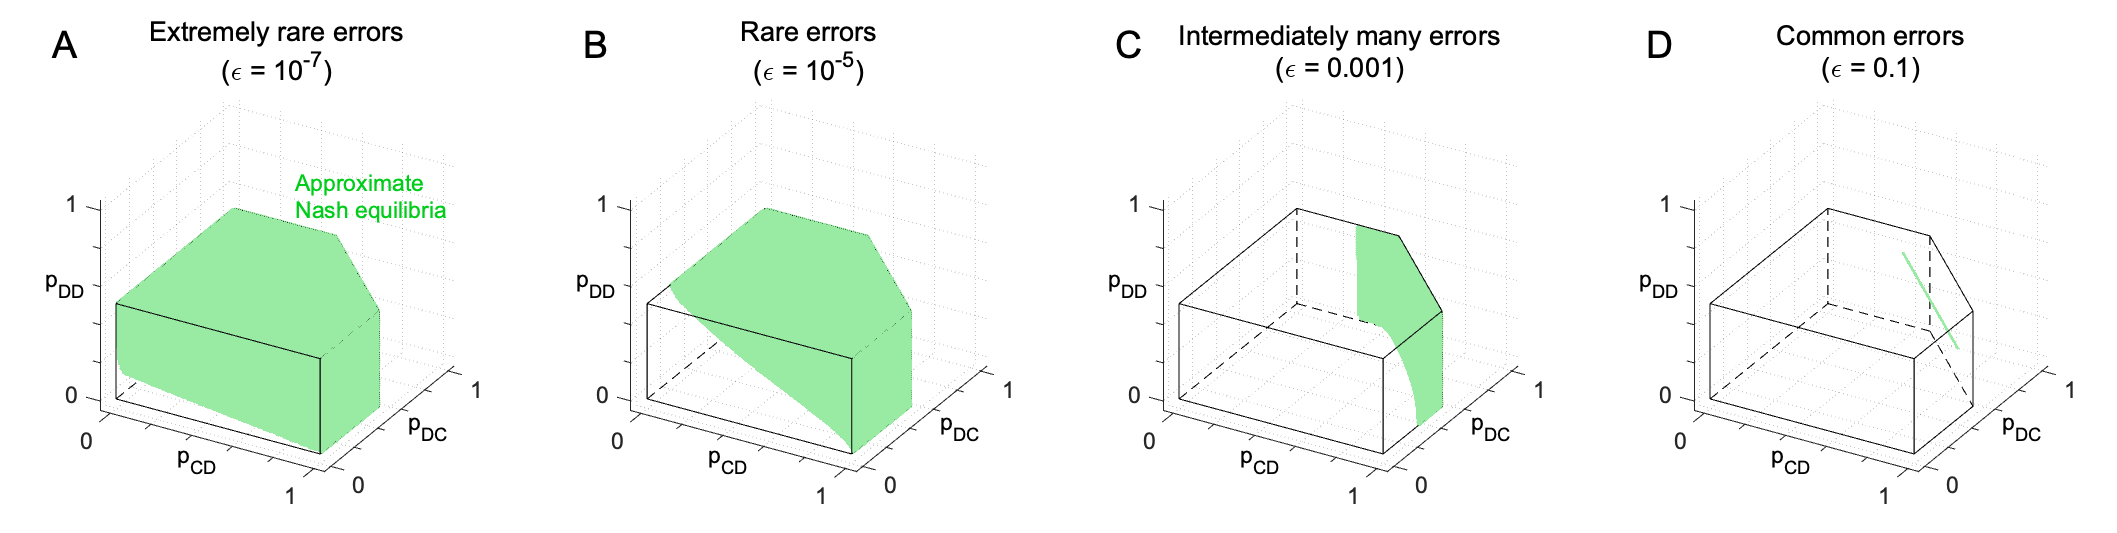
\includegraphics[width=\textwidth]{../../figures/ApproxmiateNash_strict.eps}
    \caption{{\bf The set of approximate Nash equilibria for varying error rates.} We numerically compute the set of approximate Nash equilibria among the reactive-2 strategies for the donation game (using the same parameters as in Fig.~2C of the main text). To construct this figure, we use a finite grid of self-cooperative strategies $\mathbf{p}\!=\!(1,p_{CD},p_{DC},p_{DD})$. The entries $p_{CD},p_{DC},p_{DD}$ are taken from the set $\{0,0.01,0.02,\ldots,1\}$. For each resulting strategy $\mathbf{p}$, we explore whether any pure self-reactive-2 strategy $\mathbf{\tilde p}$ satisfies $\pi^{1,\varepsilon}(\mathbf{\tilde p},\mathbf{p}) - \pi^{1,\varepsilon}(\mathbf{p},\mathbf{p}) > \Delta$. We use a comparably small value of $\Delta\!=\!0.001$, and we vary the error rate between $\varepsilon\!=\!10^{-7}$ and $\varepsilon\!=\!10^{-1}$. For sufficiently small error rates, the set of approximate partners for the game with errors approaches the set of partners for the game without errors (panel A). As we increase the error rate, the set of approximate partners approaches a line (panel D).}
    \label{fig:ApproximateNash}
\end{figure}

\subsection{Equalizers for games with implementation errors}



\clearpage
\newpage


%%%%%%%%%%%%%%%%
%%  APPENDIX: PROOFS  %%
%%%%%%%%%%%%%%%%


\section{Appendix: Proofs}
\label{section:appendix}

%%%%%%%%%%%%%%%%%%%%%%
%% APPENDIX: Proof of Akin's Lemma %% 
%%%%%%%%%%%%%%%%%%%%%%

\subsection{Proof of Lemma~\ref{lemma:AkinGeneralised}: Akin's lemma}

\begin{proof}
The proof is based on a similar argument as the proof of \eqref{Eq:EquivalencePayoff}, showing that different ways of calculating payoffs are equivalent. 
Let us first introduce some notation. 
Let $\mathbf{m^1}$ be the memory-$n$ strategy of player~1. 
For $t\!\ge\!n$ and the given strategy of player~2, let $\mathbf{v}(t)\!=\!(v_\mathbf{h})_{\mathbf{h}\in H}$ be the probability that player~1 observes the $n$-history $\mathbf{h}$ after players have made their $t$-th decision. 
By assumption, we can compute the limiting distribution
\begin{equation} \label{Eq:TimeAverageAppendix}
\mathbf{v} = \lim_{\tau\to\infty} \frac{1}{\tau} \sum_{t=n}^{n+\tau-1} \mathbf{v}(t).  
\end{equation}
Moreover, let $\rho^i(t)$ be player~i's cooperation probability in round $t$. 
For $t\!\ge\!n\!+\!1$, we obtain 
\begin{equation} \label{Eq:Rhoi}
\rho^1(t) = \big\langle \mathbf{v}(t\!-\!1) , \mathbf{m^1}\big\rangle = \big\langle \mathbf{v}(t\!+\!k\!-\!1), \mathbf{m^{k-\text{Rep}}}\big\rangle.
\end{equation}
That is, we either need to know how likely each $n$-history occurred at time $t\!-\!1$, and then we compute how likely player~1 is to cooperate in the next round, based on player 1's strategy. 
Or, we need to know how likely each $n$-history occurred after round $t\!+\!k\!-\!1$; and then we compute the correct probability by assuming player~1 cooperates in the next round if and only if the player cooperated $k$ rounds before. 
\eqref{Eq:Rhoi}~gives us two different ways to compute player~1's average payoff across all rounds,
\begin{equation}
\rho^1 := \lim_{\tau \to \infty} \frac{1}{\tau} \sum_{t=1}^\tau \rho^1(t).
\end{equation}
The first way is to take
\begin{equation*}
\begin{array}{rcl}
\rho^1 &= &\displaystyle 
\lim_{\tau \to \infty} \frac{1}{\tau} \sum_{t=1}^\tau \rho^i(t) 
= \lim_{\tau \to \infty} \frac{1}{\tau} \sum_{t=n+1}^{n+\tau} \rho^i(t)\\[0.5cm]
&= &\displaystyle 
\lim_{\tau \to \infty} \frac{1}{\tau} \sum_{t=n+1}^{n+\tau}  \big\langle \mathbf{v}(t\!-\!1) , \mathbf{m^1}\big\rangle 
=  \big\langle  \lim_{\tau \to \infty} \frac{1}{\tau} \sum_{t=n+1}^{n+\tau} \mathbf{v}(t\!-\!1) , \mathbf{m^1}\big\rangle
= \big\langle \mathbf{v},\mathbf{m^1} \big\rangle.
\end{array}
\end{equation*}
In particular, because $\big\langle \mathbf{v},\mathbf{m^1} \big\rangle$ is well-defined, so is the limiting time average~$\rho^1$. The second way is to take
\begin{equation*}
\begin{array}{rcl}
\rho^1 &= &\displaystyle 
\lim_{\tau \to \infty} \frac{1}{\tau} \sum_{t=1}^\tau \rho^i(t) 
= \lim_{\tau \to \infty} \frac{1}{\tau} \sum_{t=n+1}^{n+\tau} \rho^i(t)\\[0.5cm]
&= &\displaystyle 
\lim_{\tau \to \infty} \frac{1}{\tau} \sum_{t=n+1}^{n+\tau}  \big\langle \mathbf{v}(t\!+\!k\!-\!1) ,  \mathbf{m^{k-\text{Rep}}}\big\rangle 
=  \big\langle  \lim_{\tau \to \infty} \frac{1}{\tau} \sum_{t=n+1}^{n+\tau} \mathbf{v}(t\!+\!k\!-\!1) ,  \mathbf{m^{k-\text{Rep}}}\big\rangle
= \big\langle \mathbf{v},  \mathbf{m^{k-\text{Rep}}} \big\rangle.
\end{array}
\end{equation*}
We conclude
$
0 = \rho^1 \!-\! \rho^1 = \big\langle \mathbf{v},\mathbf{m^1} \big\rangle\!-\!\big\langle \mathbf{v},  \mathbf{m^{k-\text{Rep}}} \big\rangle\ = \big\langle \mathbf{v}, \mathbf{m^1}\!-\!\mathbf{m^{k-\text{Rep}}} \big\rangle.
$
\end{proof}




%%%%%%%%%%%%%%%%%%%%%%%%%%%%
%%  APPENDIX: Proof of  Self-Reactive Sufficiency %%
%%%%%%%%%%%%%%%%%%%%%%%%%%%% 

\subsection{Proof of Lemma~\ref{lemma:self_reactive_sufficiency}: Sufficiency of testing self-reactive strategies}

\begin{proof} 
The proof uses similar arguments as in a study by Park on alternating games~{\it et al} \citep{park:NComms:2022}. 
For the given game between player~1 (with arbitrary strategy $\sigma^1$) and player~2 (with reactive-$n$ strategy $\mathbf{p^2}$), let $v_\mathbf{h}(t)$ denote the probability to observe an $n$-history $\mathbf{h}$ at time $t\!\ge\!n$. 
By assumption, the following time averages are well-defined,
\begin{equation}\label{Eq:TimeAverageProof}
v_\mathbf{h}:=\lim_{\tau \to \infty} \frac{1}{\tau} \sum_{t=n}^{n+\tau-1} v_\mathbf{h}(t)
\end{equation}
Moreover, for any $t\!\ge\!n$ and $\mathbf{h}\!\in\! H$, let $\sigma^1_\mathbf{h}(t)$ denote the conditional probability that player~1 cooperates at time $t\!+\!1$, given the $n$-history after round $t$ is $\mathbf{h}$. Depending on $\big(\sigma^1_\mathbf{h}(t)\big)$ and $\mathbf{v}$, we define an associated self-reactive strategy $\mathbf{\tilde p^1}$ for player~1. For any given history $\mathbf{h^1} \!\in\! H^1$, the corresponding probability $\tilde p^1_\mathbf{h^1}$ is defined as an implicit solution of the equation
\begin{equation} \label{Eq:EquivalentSelfReactive}
\left( \sum_{\mathbf{h^2} \in H^2} v_{(\mathbf{h^1}, \mathbf{h^2})} \right) \tilde p^1_{\mathbf{h^1}}
=
 \sum_{\mathbf{h^2} \in H^2}
\left(\lim_{\tau \to \infty} \frac{1}{\tau} \sum_{t=n}^{n+\tau-1} v_{(\mathbf{h^1}, \mathbf{h^2})} (t)\cdot \sigma^1_{(\mathbf{h^1}, \mathbf{h^2})}(t)\right).
\end{equation}
Note that for each $\mathbf{h}\!\in\! H$, the limit in the bracket on the right hand side exists, for otherwise the limits $v_\mathbf{h}$ according to \eqref{Eq:TimeAverageProof} would not exist. Also note that if the bracket on the left hand's side is zero, the right hand side must be zero, and $\tilde p^1_\mathbf{h^1}$ can be chosen arbitrarily. Only if the bracket on the left hand side is positive, $\tilde p^1_\mathbf{h^1}$ is uniquely defined. 

We are going to show: If player~1 uses $\mathbf{\tilde p^1}$ instead of $\sigma^1$, then $\mathbf{v}$ defined by \eqref{Eq:TimeAverageProof} is an invariant distribution of the corresponding transition matrix $M$ defined by \eqref{Eq:TransitionMatrix} (hence it is also the limiting distribution of the resulting game if the first $n$ moves are chosen accordingly). For simplicity, we show the required relationship $\mathbf{v}\!=\!\mathbf{v}M$ for one of the $2^{2^n}$ equations. For the one equation we show, we consider the history according to which everyone fully cooperates, $\mathbf{h_C}\!=\!(\mathbf{h^1_C},\mathbf{ h^2_C})$. For an arbitrary $n$-history $\mathbf{h}^i=(a^i_{-n},\ldots,a^i_{-i})$, we say the $n$-history $\mathbf{\tilde h^i}=(\tilde a^i_{-n},\ldots, \tilde a^i_{-1})$ {\it is a possible successor of $\mathbf{h}$} if $\tilde a^i_{-t} = a^i_{-t+1}$ for $t\!\in\!\{2,\ldots,n\}$. To indicate successorship, we define a function $e_{\mathbf{h},\mathbf{\tilde h}}$ that is one if $\mathbf{\tilde h}$ is a possible successor of $\mathbf{h}$, and zero otherwise. 
By definition of $v_\mathbf{h}(t)$, $\sigma_\mathbf{h}^1(t)$, and $p^2_\mathbf{h}(t)$, we obtain for $t\!\ge\!n$
\begin{equation}
v_{(\mathbf{h^1_C},\mathbf{h^2_C})} (t\!+\!1)
= \sum_{\mathbf{h^1}\in H^1}\sum_{\mathbf{h^2}\in H^2} v_{(\mathbf{h^1},\mathbf{h^2})}(t)\cdot  \sigma^1_{(\mathbf{h^1},\mathbf{h^2})}(t) \cdot p^2_\mathbf{h^1} \cdot e_{\mathbf{h^1},\mathbf{h^1_C}} \cdot e_{\mathbf{h^2},\mathbf{h^2_C}}.
\end{equation}
If we sum up this equation from time $t\!=\!n$ to $t\!=\!n\!+\!\tau\!-\!1$, divide by $\tau$, and rearrange the terms, we obtain
\begin{equation}
\frac{1}{\tau}\sum_{t=n}^{n+\tau-1} v_{(\mathbf{h^1_C},\mathbf{h^2_C})} (t\!+\!1) 
= \sum_{\mathbf{h^1}\in H^1} \sum_{\mathbf{h^2}\in H^2} \left(\frac{1}{\tau}\sum_{t=n}^{n+\tau-1} v_{(\mathbf{h^1},\mathbf{h^2})}(t)\cdot  \sigma^1_{(\mathbf{h^1},\mathbf{h^2})}(t)\right) \cdot p^2_\mathbf{h^1} \cdot e_{\mathbf{h^1},\mathbf{h^1_C}} \cdot e_{\mathbf{h^2},\mathbf{h^2_C}}.
\end{equation}
Taking the limit $\tau\to\infty$, and taking into account the relationships~\eqref{Eq:TimeAverageProof} and \eqref{Eq:EquivalentSelfReactive}, this simplifies to
\begin{equation} 
v_{(\mathbf{h^1_C},\mathbf{h^2_C})}
= \sum_{\mathbf{h^1}\in H^1}\sum_{\mathbf{h^2} \in H^2} v_{(\mathbf{h^1}, \mathbf{h^2})} \cdot \big(\tilde p^1_{\mathbf{h^1}} \, e_{\mathbf{h^1},\mathbf{h^1_C}}\big) \cdot \big(p^2_\mathbf{h^1} \, e_{\mathbf{h^2},\mathbf{h^2_C}}\big).
\end{equation}
By using the definition of transition probabilities in~\eqref{Eq:TransitionMatrix}, this expression further simplifies to
\begin{equation} 
v_\mathbf{h_C} = \sum_{\mathbf{h}} v_{\mathbf{h}} \cdot M_{\mathbf{h},\mathbf{h_C}}
\end{equation}
That is, out of the $2^{2n}$ individual equations in the linear system $\mathbf{v}\!=\!\mathbf{v} M$, we have verified the equation for the probability to observe full cooperation $\mathbf{h_C}$ after one round. All other equations follow analogously.
\end{proof}


%%%%%%%%%%%%%%%%%%%%%%%%%%%%
%%  APPENDIX: Proof of  Self-Reactive Sufficiency %%
%%%%%%%%%%%%%%%%%%%%%%%%%%%% 

\subsection{Proof of Lemma~\ref{lemma:self_reactive_sufficiency}: Sufficiency of testing self-reactive strategies}

\begin{proof} 
The proof uses similar arguments as in a study by Park on alternating games~{\it et al} \citep{park:NComms:2022}. 
For the given game between player~1 (with arbitrary strategy $\sigma^1$) and player~2 (with reactive-$n$ strategy $\mathbf{p^2}$), let $v_\mathbf{h}(t)$ denote the probability to observe an $n$-history $\mathbf{h}$ at time $t\!\ge\!n$. 
By assumption, the following time averages are well-defined,
\begin{equation}\label{Eq:TimeAverageProof}
v_\mathbf{h}:=\lim_{\tau \to \infty} \frac{1}{\tau} \sum_{t=n}^{n+\tau-1} v_\mathbf{h}(t)
\end{equation}
Moreover, for any $t\!\ge\!n$ and $\mathbf{h}\!\in\! H$, let $\sigma^1_\mathbf{h}(t)$ denote the conditional probability that player~1 cooperates at time $t\!+\!1$, given the $n$-history after round $t$ is $\mathbf{h}$. Depending on $\big(\sigma^1_\mathbf{h}(t)\big)$ and $\mathbf{v}$, we define an associated self-reactive strategy $\mathbf{\tilde p^1}$ for player~1. For any given history $\mathbf{h^1} \!\in\! H^1$, the corresponding probability $\tilde p^1_\mathbf{h^1}$ is defined as an implicit solution of the equation
\begin{equation} \label{Eq:EquivalentSelfReactive}
\left( \sum_{\mathbf{h^2} \in H^2} v_{(\mathbf{h^1}, \mathbf{h^2})} \right) \tilde p^1_{\mathbf{h^1}}
=
 \sum_{\mathbf{h^2} \in H^2}
\left(\lim_{\tau \to \infty} \frac{1}{\tau} \sum_{t=n}^{n+\tau-1} v_{(\mathbf{h^1}, \mathbf{h^2})} (t)\cdot \sigma^1_{(\mathbf{h^1}, \mathbf{h^2})}(t)\right).
\end{equation}
Note that for each $\mathbf{h}\!\in\! H$, the limit in the bracket on the right hand side exists, for otherwise the limits $v_\mathbf{h}$ according to Eq.~\eqref{Eq:TimeAverageProof} would not exist. Also note that if the bracket on the left hand's side is zero, the right hand side must be zero, and $\tilde p^1_\mathbf{h^1}$ can be chosen arbitrarily. Only if the bracket on the left hand side is positive, $\tilde p^1_\mathbf{h^1}$ is uniquely defined. 

We are going to show: If player~1 uses $\mathbf{\tilde p^1}$ instead of $\sigma^1$, then $\mathbf{v}$ defined by Eq.~\eqref{Eq:TimeAverageProof} is an invariant distribution of the corresponding transition matrix $M$ defined by Eq.~\eqref{Eq:TransitionMatrix} (hence it is also the limiting distribution of the resulting game if the first $n$ moves are chosen accordingly). For simplicity, we show the required relationship $\mathbf{v}\!=\!\mathbf{v}M$ for one of the $2^{2^n}$ equations. For the one equation we show, we consider the history according to which everyone fully cooperates, $\mathbf{h_C}\!=\!(\mathbf{h^1_C},\mathbf{ h^2_C})$. For an arbitrary $n$-history $\mathbf{h}^i=(a^i_{-n},\ldots,a^i_{-i})$, we say the $n$-history $\mathbf{\tilde h^i}=(\tilde a^i_{-n},\ldots, \tilde a^i_{-1})$ {\it is a possible successor of $\mathbf{h}$} if $\tilde a^i_{-t} = a^i_{-t+1}$ for $t\!\in\!\{2,\ldots,n\}$. To indicate successorship, we define a function $e_{\mathbf{h},\mathbf{\tilde h}}$ that is one if $\mathbf{\tilde h}$ is a possible successor of $\mathbf{h}$, and zero otherwise. 
By definition of $v_\mathbf{h}(t)$, $\sigma_\mathbf{h}^1(t)$, and $p^2_\mathbf{h}(t)$, we obtain for $t\!\ge\!n$
\begin{equation}
v_{(\mathbf{h^1_C},\mathbf{h^2_C})} (t\!+\!1)
= \sum_{\mathbf{h^1}\in H^1}\sum_{\mathbf{h^2}\in H^2} v_{(\mathbf{h^1},\mathbf{h^2})}(t)\cdot  \sigma^1_{(\mathbf{h^1},\mathbf{h^2})}(t) \cdot p^2_\mathbf{h^1} \cdot e_{\mathbf{h^1},\mathbf{h^1_C}} \cdot e_{\mathbf{h^2},\mathbf{h^2_C}}.
\end{equation}
If we sum up this equation from time $t\!=\!n$ to $t\!=\!n\!+\!\tau\!-\!1$, divide by $\tau$, and rearrange the terms, we obtain
\begin{equation}
\frac{1}{\tau}\sum_{t=n}^{n+\tau-1} v_{(\mathbf{h^1_C},\mathbf{h^2_C})} (t\!+\!1) 
= \sum_{\mathbf{h^1}\in H^1} \sum_{\mathbf{h^2}\in H^2} \left(\frac{1}{\tau}\sum_{t=n}^{n+\tau-1} v_{(\mathbf{h^1},\mathbf{h^2})}(t)\cdot  \sigma^1_{(\mathbf{h^1},\mathbf{h^2})}(t)\right) \cdot p^2_\mathbf{h^1} \cdot e_{\mathbf{h^1},\mathbf{h^1_C}} \cdot e_{\mathbf{h^2},\mathbf{h^2_C}}.
\end{equation}
Taking the limit $\tau\to\infty$, and taking into account the relationships~\eqref{Eq:TimeAverageProof} and \eqref{Eq:EquivalentSelfReactive}, this simplifies to
\begin{equation} 
v_{(\mathbf{h^1_C},\mathbf{h^2_C})}
= \sum_{\mathbf{h^1}\in H^1}\sum_{\mathbf{h^2} \in H^2} v_{(\mathbf{h^1}, \mathbf{h^2})} \cdot \big(\tilde p^1_{\mathbf{h^1}} \, e_{\mathbf{h^1},\mathbf{h^1_C}}\big) \cdot \big(p^2_\mathbf{h^1} \, e_{\mathbf{h^2},\mathbf{h^2_C}}\big).
\end{equation}
By using the definition of transition probabilities in~\eqref{Eq:TransitionMatrix}, this expression further simplifies to
\begin{equation} 
v_\mathbf{h_C} = \sum_{\mathbf{h}} v_{\mathbf{h}} \cdot M_{\mathbf{h},\mathbf{h_C}}
\end{equation}
That is, out of the $2^{2n}$ individual equations in the linear system $\mathbf{v}\!=\!\mathbf{v} M$, we have verified the equation for the probability to observe full cooperation $\mathbf{h_C}$ after one round. All other equations follow analogously.
\end{proof}





%%%%%%%%%%%%%%%%%%%%%%%%%%%%%%
%%  APPENDIX: Proof of pure self-reactive Sufficiency %%
%%%%%%%%%%%%%%%%%%%%%%%%%%%%%%

\subsection{Proof of Theorem~\ref{theorem:nash_against_pure_self_reactive}: Sufficiency of pure self-reactive strategies}

By Lemma~\ref{lemma:self_reactive_sufficiency}, there exists a best response to $\mathbf{p}$ within the self-reactive $n$ strategies. 
It remains to show that this best response $\mathbf{\tilde p}$ can be chosen to be pure. 
The proof follows from a series of auxiliary results. 
The first such result uses an insight by Press \& Dyson~\citep{press:PNAS:2012}. 
They showed that given the transition matrix of a game among two memory-1 players, one can compute the players' payoffs by considering determinants of certain associated matrices. 
Herein, we apply their method to the transition matrix $\tilde M\!=\!(\tilde M_{\mathbf{h},\mathbf{h'}})$ according to Eq.~\eqref{Eq:TransitionMatrixSelfReactive} for a given self-reactive strategy $\mathbf{\tilde p}\!\in\!\mathcal{S}_n$. 
For some fixed $n$-history $\mathbf{h'}$, we define an associated matrix $\tilde M_\mathbf{h'}$ that one obtains from  $\tilde M$ with the following two steps:
\begin{enumerate}
\item Subtract the $2^n\!\times\!2^n$ identity matrix $I$ from $\tilde M$. 
\item In the resulting matrix, replace the last column by a column that only contains zeros, except for the row corresponding to the history $\mathbf{h'}$, for which the entry is one. 
\end{enumerate}
These matrices $\tilde M_\mathbf{h'}$ can be used to compute the invariant distribution of the original matrix $\tilde M$ as follows.\\

\noindent
{\bf Auxiliary result 1:}
Let $\mathbf{\tilde p}\!\in\!\mathcal{S}_n$ be such that its transition matrix $\tilde M$ according to Eq.~\eqref{Eq:TransitionMatrixSelfReactive} has a unique invariant distribution $\mathbf{\tilde v} \!=\! (\tilde v_\mathbf{h^1})_{\mathbf{h^1}\in H^1}$. Then for all $\mathbf{h'}\!\in\!H^1$ we have
\begin{equation} \label{Eq:PDFormula}
\tilde v_\mathbf{h'} = \frac{ \det(\tilde M_{\mathbf{h'}})}{ \sum_{\mathbf{h^1}\in H^1} \det(\tilde M_{\mathbf{h^1}})}.
\end{equation}

\begin{proof}[Proof of Auxiliary result~1]
The result follows from Press \& Dyson's formula for the dot product of the invariant distribution $\mathbf{\tilde v}$ with an arbitrary vector $\mathbf{f}$, by taking the vector $\mathbf{f}$ to be the unit vector with only the entry for history $\mathbf{h'}$ being one. 
\end{proof}

\noindent
Based on this first auxiliary result, we have an explicit representation of the payoff function $\pi^1(\mathbf{\tilde p},\mathbf{p})$ that describes the payoff of a self-reactive player with strategy $\mathbf{\tilde p}$ against a reactive player with strategy $\mathbf{p}$. 
Specifically, by plugging Eq.~\eqref{Eq:PDFormula} into \eqref{eq:PD_long_term_payoff}, we obtain
\begin{equation} \small
\pi^1(\mathbf{\tilde p},\mathbf{p}) \!=\frac{\sum_{\mathbf{h^1}\in H^1}\det(\tilde M_\mathbf{h^1})
\Big(
\mathbf{\tilde p}_\mathbf{h^1} \mathbf{p}_\mathbf{h^1}\!\cdot\!R +
\mathbf{\tilde p}_\mathbf{h^1} (1\!-\!\mathbf{p}_\mathbf{h^1})\!\cdot\!S +  
(1\!-\!\mathbf{\tilde p}_\mathbf{h^1}) \mathbf{p}_\mathbf{h^1}\!\cdot\!T +
(1\!-\!\mathbf{\tilde p}_\mathbf{h^1}) (1\!-\!\mathbf{p}_\mathbf{h^1})\!\cdot\!P 
\Big)}
{\sum_{\mathbf{h^1}\in H^1} \det(\tilde M_{\mathbf{h^1}})}.
\end{equation}
For our purposes, the following properties of this payoff function will be important.\\

\noindent
{\bf Auxiliary Result 2:}
On its domain, the payoff function $\pi^1(\mathbf{\tilde p},\mathbf{p})$ is a bounded rational function, and both its numerator and denominator are linear in each entry $\tilde p_\mathbf{h^i} $, for all $\mathbf{h^i}\!\in\!H^i$.

\begin{proof}[Proof of Auxiliary Result~2]
By its definition, each $\det(\tilde M_\mathbf{h^i})$ is a polynomial. Moreover, because for each history $\mathbf{h'}$, the cooperation probability $\tilde p_\mathbf{h'}$ only appears in a single row of $\tilde M_\mathbf{h^i}$ (and there it appears linearly), it also appears linearly in  $\det(\tilde M_\mathbf{h^i})$. Finally, we note that $\det(\tilde M_\mathbf{h^i})$ does not depend on $\tilde p_\mathbf{h^i}$. To see this, we can compute $\det(\tilde M_\mathbf{h^i})$ using Laplace expansion along the last column. As a result, we obtain that this determinant is up to its sign equal to the determinant of the matrix one obtains from $\tilde M_\mathbf{h^i}$ by deleting the last column, and the row $\mathbf{h^i}$ (which is the only row of $\tilde M_\mathbf{h^i}$ that contains $\tilde p_\mathbf{h^i}$). 

Finally, we note that the payoff function is bounded, because as an average payoff per round, payoffs need to be between $T$ and $S$. Taken together, these observations imply the result for $\pi^1(\mathbf{\tilde p},\mathbf{p})$. 
\end{proof}

\noindent
The following result describes a useful property of bounded linear rational functions.\\

\noindent
{\bf Auxiliary Result 3:} Suppose $g,h:[0,1]^{k}\!\rightarrow\! \mathbb{R}$ and suppose both $g(\mathbf{x})$ and $h(\mathbf{x})$ are linear in each component of $\mathbf{x}\!=\!(x_1,\ldots,x_k)$. 
Moreover, suppose $f\!:=\!g/h$ is bounded on $[0,1]^{k}$. 
For a given $\mathbf{x}$ and $j\!\in\!\{1,\ldots,k\}$, we define an associated function $f_{\mathbf{x},j}:[-x_j,1\!-\!x_j]\to\mathbb{R}$ by only varying the $j$-th component, $f_{\mathbf{x},j}(t) = f(x_1,\ldots,x_j+t,\ldots,x_k)$. Then for all $\mathbf{x}\!\in\![0,1]^k$ and $j$, the function  $f_{\mathbf{x},j}(t)$ is either monotonically increasing, monotonically decreasing, or constant.

\begin{proof}[Proof of Auxiliary Result 3]
Let $g(\mathbf{x}):=a_0\!+\!a_1x_1\!+\!\ldots \!+\!a_k x_k$ and $h(\mathbf{x}):=b_0\!+\!b_1x_1\!+\!\ldots \!+\!b_k x_k$, and consider some arbitrary but fixed $\mathbf{x}\!\in\![0,1]^k$ and $j$. We compute
\begin{equation}
f'_{\mathbf{x},j}(t) = \frac{\partial}{\partial t}  f(x_1,\ldots,x_j+t,\ldots,x_k) = \frac{a_j\left( \sum_{i\neq j} b_i x_i\right) - b_j \left(\sum_{i\neq j} a_i x_i\right)}{\big(b_0+b_1x_1+\ldots+b_j(x_j+t)+\ldots+b_kx_k\big)^2}.
\end{equation}
Because $f$ is bounded on the entire domain, the denominator in this expression for $f'_{\mathbf{x},j}(t)$ is strictly positive. Moreover, we note that the numerator is independent of $t$. Thus, depending on the sign of the numerator, $f'_{\mathbf{x},j}(t)$ is either monotonically increasing, monotonically decreasing, or constant. 
\end{proof}

\noindent
After these preparations, we are ready to prove the main result. 

\begin{proof}[Proof of Theorem~\ref{theorem:nash_against_pure_self_reactive}]
For a given reactive strategy $\mathbf{p}\!\in\!\mathcal{R}_n$, let the self-reactive $\mathbf{\tilde p}\!\in\!\mathcal{S}_n$ be a best response. Suppose there is some history $\mathbf{h'}$ such that $0\!<\!\tilde p_\mathbf{h}\!<\!1$. It follows from the Auxiliary Results 2~and~3 that $\pi^1(\mathbf{\tilde p},\mathbf{p})$ is either monotonically increasing, monotonically decreasing, or constant in $\tilde p_\mathbf{h'}$. 
If it was increasing or decreasing, we end up with a contradiction, because no local improvement should be possible for a best response. 
Therefore, $\pi^1(\mathbf{\tilde p},\mathbf{p})$  must be independent of $\tilde p_\mathbf{h'}$, and hence we can set 
$\tilde p_\mathbf{h'}\!=\!0$ or $\tilde p_\mathbf{h'}\!=\!1$ without changing $\pi^1(\mathbf{\tilde p},\mathbf{p})$. By iteratively applying this reasoning to all histories $\mathbf{h}$ for which $0\!<\!\tilde p_\mathbf{h}\!<\!1$, we obtain the desired result. 
\end{proof}



%%%%%%%%%%%%%%%%%%%%%%%%%%%%%%
%%  APPENDIX:  Reactive-2 partners, donation game  %%
%%%%%%%%%%%%%%%%%%%%%%%%%%%%%%

\subsection{Proof of Theorem~\ref{theorem:reactive_two_partner_strategies}: Reactive-2 partner strategies in the donation game}
\begin{proof}
Given that player~1 uses a nice reactive-2 strategy $\mathbf{p} = (1, p_{CD},p_{DC}, p_{DD})$, the claim is true if and only if it is true for all deviation towards the sixteen pure self-reactive-2 strategies $\mathbf{\tilde{p}}\!\in\!\{0,1\}^{16}$. 
In the following, we enumerate these sixteen strategies, $\{\mathbf{\tilde{p}_0}, \dots, \mathbf{\tilde{p}_{15}}\}$, 
by interpreting them as binary numbers, 
\begin{equation}
\mathbf{\tilde p} = (\tilde p_{CC}, \tilde p_{CD},\tilde p_{DC},\tilde p_{DD}) ~\mapsto~
\tilde p_{CC} \!\cdot\! 2^3 + \tilde p_{CD} \!\cdot\! 2^2 + \tilde p_{DC} \!\cdot\! 2^1 + p_{DD}\cdot 2^0. 
\end{equation}
In particular, \alld{} $=\!(0,0,0,0)$ is mapped to the number $j\!=\!0$, and \allc{} $=\!(1,1,1,1)$ is mapped to $j\!=\!15$. 
The possible payoffs against the reactive strategy $\mathbf{p}$ can be computed by \eqref{eq:PD_long_term_payoff}, which yields
\begin{equation*}\label{Eq:PayoffExpressionsReactiveTwo}
  \begin{array}{lcll}
   \pi^1(\mathbf{\tilde p_j},\mathbf{p}) &= &\displaystyle p_{DD}\cdot b & ~~\text{for}~ j\! \in\!  \{0, 2, 4, 6, 8, 10, 12, 14\} \\[0.3cm]
   \pi^1(\mathbf{\tilde p_j},\mathbf{p}) &= &\displaystyle  \frac{p_{CD} + p_{DC} + p_{DD}}{3}\cdot b - \frac{1}{3} \cdot c  & ~~\text{for}~ j\! \in\!  \{1, 9\} \\[0.3cm]
   \pi^1(\mathbf{\tilde p_j},\mathbf{p}) &= &\displaystyle  \frac{1+p_{CD} + p_{DC} + p_{DD} }{4}\cdot b - \frac{1}{2} \cdot c  & ~~\text{for}~ j\! \in\!  \{3\} \\[0.3cm]
   \pi^1(\mathbf{\tilde p_j},\mathbf{p}) &= &\displaystyle  \frac{p_{CD} + p_{DC}}{2}\cdot b - \frac{1}{2} \cdot c  & ~~\text{for}~ j\! \in\!  \{4, 5, 12, 13\} \\[0.3cm]
   \pi^1(\mathbf{\tilde p_j},\mathbf{p}) &= &\displaystyle  \frac{1+p_{CD} + p_{DC}}{3}\cdot b - \frac{2}{3} \cdot c  & ~~\text{for}~ j\! \in\!  \{6, 7\}\\[0.3cm]
   \pi^1(\mathbf{\tilde p_j},\mathbf{p}) &= &\displaystyle  b - c & ~~\text{for}~ j\! \in\!  \{8, 9, 10, 11, 12, 13, 14, 15\}
  \end{array}
\end{equation*}
In this list, some strategy indices $j$ appear multiple times. 
Those instances correspond to strategies that have multiple invariant distributions (such as the strategy 1-round repeat, with $j\!=\!10$). For those strategies, we have computed the payoffs for all possible initial $n$-histories.  
Requiring the payoffs in this list to be at most the mutual cooperation payoff $b\! -\! c$, we get the following unique conditions,
\begin{equation*}
 p_{DD}  \le 1 \!-\! \frac{c}{b}, \qquad \qquad
\frac{p_{CD} + p_{DC}}{2}  \le 1\! -\! \frac{1}{2} \,  \frac{c}{b}, \qquad \qquad
 \frac{p_{CD} + p_{DC} + p_{DD}}{3} \le	 1 \!-\! \frac{2}{3} \, \frac{c}{b}.
\end{equation*}
Because the last condition is implied by the first two, we end up with the conditions in~\eqref{eq:two_bit_conditions}. 
\end{proof}



%%%%%%%%%%%%%%%%%%%%%%%%%%%%%%
%%  APPENDIX:  Reactive-3 partners, donation game  %%
%%%%%%%%%%%%%%%%%%%%%%%%%%%%%%

\subsection{Proof of Theorem~\ref{theorem:reactive_three_partner_strategies}: Reactive-3 partner strategies in the donation game}

\begin{proof}
The proof is similar to the previous one. 
Again, enumerating the 256 pure self-reactive 3 strategies $\mathbf{\tilde p}$ by interpreting the strategy as a binary number, we obtain the following payoffs. 
\begin{equation*}\label{Eq:PayoffExpressionsReactiveThree}
\footnotesize
\setlength{\arraycolsep}{0mm}
\begin{array}{lclll}
\pi^1(\mathbf{\tilde p_j},\mathbf{p}) &{\, = \,}
&\displaystyle b \; p_{DDD} 
&~\text{for}~ j\! \in\! 
&\{0, 2, 4, 6, \dots, 250, 252, 254\} \\[0.2cm]

\pi^1(\mathbf{\tilde p_j},\mathbf{p}) &= 
&\displaystyle \frac{p_{CDD} \!+\! p_{DCD}\!+\!  p_{DDC} \!+\!  p_{DDD}}{4}\,b - \frac{1}{4}\,c 
&~\text{for}~ j\! \in\!  
& \{ 1, 9, 33, 41, 65, 73, 97, 105, 129, 137, 161,
	\\ & & &  &169, 193, 201, 225, 233\} \\[0.2cm]
    
\pi^1(\mathbf{\tilde p_j},\mathbf{p}) &= 
&\displaystyle \frac{p_{CCD} \!+\! p_{CDD} \!+\! p_{DCC} \!+\! p_{DDC} \!+\! p_{DDD}}{5}\,b - \frac{2}{5} \, c &~\text{for}~ j\! \in\!  
& \{ 3, 7, 35, 39, 131, 135, 163, 167\} \\[0.2cm]

\pi^1(\mathbf{\tilde p_j},\mathbf{p}) &= 
&\displaystyle \frac{p_{CDC} \!+\! p_{DCD}}{2}\,b - \frac{1}{2} \, c 
&~\text{for}~ j\! \in\!  
& \{ 4 \!- \!7, 12 \!- \!15, 20 \!- \!23, 28 \!- \!31, 68 \!- \!71,
    \\ & & &  &76 \!- \!79, 84 \!- \!87, 92 \!- \!95, 132 \!- \!135, 
    \\ & & & &140 \!- \!143, 148- 151, 156 \!- \!159, 
    \\ & & & &196 \!- \!199, 204 \!- \!207, 212 \!- \!215, 220 \!- \!223\} \\[0.2cm]
    
\pi^1(\mathbf{\tilde p_j},\mathbf{p}) &= 
&\displaystyle \frac{1\!+\!p_{CCD} \!+\! p_{CDD} \!+\! p_{DCC} \!+\! p_{DDC} \!+\! p_{DDD}}{6}\,b - \frac{1}{2} \, c 
&~\text{for}~ j\! \in\! 
& \{ 11, 15, 43, 47\} \\ [0.2cm]

\pi^1(\mathbf{\tilde p_j},\mathbf{p}) &= 
&\displaystyle \frac{p_{CDD} \!+\! p_{DCD} \!+\! p_{DDC}}{3}\,b - \frac{1}{3} \, c 
&~\text{for}~ j\! \in\! 
& \{16,17,24,25,48,49,56,57,80,81,88,
    \\ & & & &89,112, 113,120,121, 144,145,152,153,
    \\ & & & &176,177,184,185,208,209,216,217,
    \\ & & & &240, 241,248,249\} \\[0.2cm]
    
\pi^1(\mathbf{\tilde p_j},\mathbf{p}) &= 
&\displaystyle \frac{p_{CCD} \!+\! p_{CDD} \!+\! p_{DCC} \!+\! p_{DDC}}{4}\,b - \frac{1}{2} \, c 
&~\text{for}~ j\! \in\! 
& \{ 18, 19, 22, 23, 50, 51, 54, 55, 146, 147,
    \\ & & &  &150, 151, 178, 179, 182, 183\} \\[0.2cm]
    
\pi^1(\mathbf{\tilde p_j},\mathbf{p}) &= 
&\displaystyle \frac{1 \!+\! p_{CCD} \!+\! p_{CDD} \!+\! p_{DCC} \!+\! p_{DDC}}{5}\, b - \frac{3}{5} \, c 
&~\text{for}~ j\! \in\! 
& \{ 26, 27, 30, 31, 58, 59, 62, 63\} \\ [0.2cm]

\pi^1(\mathbf{\tilde p_j},\mathbf{p}) &= 
&\displaystyle \frac{p_{CCD} \!+\! p_{CDC} \!+\! p_{CDD} \!+\! p_{DCC} \!+\! p_{DCD} \!+\! p_{DDC} \!+\! p_{DDD}}{7} \,b - \frac{3}{7} \, c
&~\text{for}~ j\! \in\! 
& \{ 37, 67, 165, 195\} \\ [0.2cm]

\pi^1(\mathbf{\tilde p_j},\mathbf{p}) &= 
&\displaystyle \frac{1 \!+\! p_{CCD} \!+\! p_{CDC} \!+\! p_{CDD} \!+\! p_{DCC} \!+\! p_{DCD} \!+\! p_{DDC} \!+\! p_{DDD}}{8}\,b - \frac{1}{2} \, c~~~~~
&~\text{for}~ j\! \in\! 
& \{ 45, 75\} \\ [0.2cm]

\pi^1(\mathbf{\tilde p_j},\mathbf{p}) &= 
&\displaystyle \frac{p_{CCD} \!+\! p_{CDC} \!+\! p_{CDD} \!+\! p_{DCC} \!+\! p_{DCD} \!+\! p_{DDC}}{6}\,b - \frac{1}{2} \, c 
&~\text{for}~ j\! \in\! 
& \{ 52, 53, 82, 83, 180, 181, 210, 211\} \\  [0.2cm]

\pi^1(\mathbf{\tilde p_j},\mathbf{p}) &= 
&\displaystyle \frac{1 \!+\! p_{CCD} \!+\! p_{CDC} \!+\! p_{CDD} \!+\! p_{DCC} \!+\! p_{DCD} \!+\! p_{DDC}}{7}\,b - \frac{4}{7} \, c 
&~\text{for}~ j\! \in\! 
& \{ 60, 61, 90, 91\} \\ [0.2cm]

\pi^1(\mathbf{\tilde p_j},\mathbf{p}) &= 
&\displaystyle \frac{p_{CCD} \!+\! p_{CDC} \!+\! p_{DCC}}{3}\,b - \frac{2}{3} \, c 
&~\text{for}~ j\! \in\! 
& \{ 96\!- \!103, 112\!- \!119, 224\!- \!231, 240\!- \!247\} \\ [0.2cm]
    
\pi^1(\mathbf{\tilde p_j},\mathbf{p}) &= 
&\displaystyle \frac{1\!+\!p_{CCD} \!+\! p_{CDC} \!+\! p_{DCC}}{4}\,b - \frac{3}{4} \, c 
&~\text{for}~ j\! \in\! 
& \{ 104\!-\!111, 120\!- \!127\} \\ [0.2cm]

\pi^1(\mathbf{\tilde p_j},\mathbf{p}) &= 
&\displaystyle b - c 
&~\text{for}~ j\! \in\! 
& \{128, 129, 130, \dots, 255\}
\end{array}
\end{equation*}

\noindent
Requiring these payoffs to be at most  equal to the mutual cooperation payoff $b\!-\!c$
gives
\begin{equation*} \footnotesize
\begin{array}{c}
\displaystyle  p_{DDD} \leq 1 \!- \!\frac{c}{b}, 
  \qquad \qquad \frac{p_{CDC} + p_{DCD}}{2} \leq 1 - \frac{1}{2} \cdot \frac{c}{b}, 
  \qquad \qquad \frac{p_{CDD} + p_{DCD} + p_{DDC}}{3} \leq 1 - \frac{2}{3} \cdot \frac{c}{b},\\[0.45cm]
\displaystyle  \frac{p_{CCD} + p_{CDC} + p_{DCC}}{3} \leq 1 - \frac{1}{3} \cdot \frac{c}{b},
  \quad \qquad \frac{p_{CCD} + p_{CDD} + p_{DCC} + p_{DDC}}{4} \leq 1 - \frac{1}{2}  \cdot \frac{c}{b}, \\[0.45cm]
\displaystyle  \frac{p_{CDD} + p_{DCD} + p_{DDC} + p_{DDD}}{4} \leq 1 - \frac{3}{4} \cdot \frac{c}{b}, 
  \quad \qquad \frac{p_{CCD} + p_{CDC} + p_{CDD} + p_{DCC} + p_{DCD} + p_{DDC} + p_{DDD}}{7} \leq 1 - \frac{4}{7} \cdot \frac{c}{b}, \\[0.45cm]
\displaystyle  \frac{p_{CCD} + p_{CDD} + p_{DCC} + p_{DDC} + p_{DDD}}{5} \leq 1 - \frac{3}{5} \cdot \frac{c}{b},
  \quad \qquad \frac{p_{CCD} + p_{CDC} + p_{CDD} + p_{DCC} + p_{DCD} + p_{DDC}}{6} \leq 1 - \frac{1}{2} \cdot \frac{c}{b}.
  \end{array}
\end{equation*}
The statement follows by noting that the five conditions in the first two rows imply the four other conditions.
\end{proof}



%%%%%%%%%%%%%%%%%%%%%%%%%%
%%  APPENDIX:  Reactive-n counting partners  %%
%%%%%%%%%%%%%%%%%%%%%%%%%%


\subsection{Proof of Theorem~\ref{theorem:reactive_counting_partner_strategies}: Reactive-$n$ counting strategies in the donation game}

Before we go into the details of the proof, we first start with two useful observations.

\begin{enumerate}
\item Assume player~1 adopts a given self-reactive strategy $\mathbf{\tilde p}$ and player~2 adopts the reactive-$n$ strategy $\mathbf{r}\!=\!(r_k)_{k\in\{n,\ldots,0\}}$. For the resulting game, suppose $\mathbf{v}$ is the limiting distribution according to \eqref{Eq:TimeAverage}. 
Then it is useful to express $\mathbf{v}$ in terms of what the counting player can remember. To this end, let $H^1_k$ be the set of $n$-histories according to which player 1 has cooperated exactly $k$ times,
\begin{equation}
H^1_k = \Big\{ \mathbf{h^1} \!\in\! H^1~\Big|~|\mathbf{h^1}|\!=\!k~\Big\}.
\end{equation}
Accordingly, let $\mathbf{u}\!=\!(u_k)_{k\in\{0,\ldots,n\}}$ be the distribution that summarizes how often, on average, player~1 cooperates $j$ times during $n$ consecutive rounds, 
\begin{equation}
u^1_k = \sum_{\mathbf{h^1} \in H^1_k} v_\mathbf{h^1}.
\end{equation}
In particular, the entries of $\mathbf{u}$ are normalized, 
\begin{equation} \label{Eq:uNormalized}
\sum_{k=0}^n u^1_k = 1. 
\end{equation}
Moreover, the average cooperation rate of the two players can be written as
\begin{equation}
\rho^1 = \sum_{k=0}^n \frac{k}{n}\,u^1_k \qquad \text{and} \qquad \rho^2 = \sum_{k=0}^n r_k\,u^1_k.
\end{equation}
Because payoffs in the donation game only depend on the players' average cooperation rates (but not on the timing of cooperation), we conclude that player 1's payoff is
\begin{equation} \label{Eq:CountingDeviationPayoff}
\pi^1(\mathbf{\tilde p},\mathbf{r}) = \sum_{k=0}^n  (r_k\,b - \frac{k}{n}\,c) \,u^1_k.
\end{equation}

\item There is a set of strategies for which payoffs are particularly easy to compute. 
We refer to them as simple periodic strategies, $\sigma_{k}$ with $k\!\in\!\{0,\ldots,n\}$. 
A player with strategy $\sigma_{k}$ cooperates in round $t$ if and only if 
\begin{equation} \label{Eq:SimplePeriodic}
t-1\!\!\mod n < k.
\end{equation}
That is, such a player cooperates in the first $k$ rounds, then defects for $n\!-\!k$ rounds, then cooperates for another $k$ rounds, only to defect in the $n\!-\!k$ subsequent rounds, etc. 
Such strategies are interesting for two reasons. 
First, they all can be interpreted as a round-$n$ repeat strategy $\mathbf{\tilde p^{n-\text{Rep}}}$, as defined by~\eqref{Eq:Repeat}.
During the initial $n$ rounds, they cooperate according to \eqref{Eq:SimplePeriodic}; thereafter, they simply repeat whatever they have done $n$ rounds ago. 
Second, players with  strategy $\sigma_{k}$ always act in such a way that according to any resulting $n$-history, they have cooperated exactly $k$ times during the last $n$ rounds. As a result, if player~1 adopts such a strategy in a donation game against a player with a reactive-$n$ counting strategy~$\mathbf{r}$, then player 1's average payoff is 
\begin{equation} \label{Eq:PaySimplePeriodic}
\pi^1(\sigma_{k},\mathbf{r}) = r_k\,b - \frac{k}{n}\,c.
\end{equation}
\end{enumerate}

\noindent
After these observations, we are ready for the actual proof. 

\begin{proof}[Proof of Theorem~\ref{theorem:reactive_counting_partner_strategies}] ~
\begin{description}
\item[\normalfont ($\Rightarrow$)]
Suppose the reactive-$n$ counting strategy $\mathbf{r}$ is a partner.
Because it is nice, it cooperates against an unconditional cooperator, and hence $r_n\!=\!1$. 
Because it is a Nash equilibrium, player~1 must not have an incentive to deviate towards any of the simple periodic strategies $\sigma_k$. By \eqref{Eq:PaySimplePeriodic}, this means that for all $k\!\in\!\{0,\ldots,n\}$ we have
\begin{equation}
 r_k\,b - \frac{k}{n}\,c \le b\!-\!c.
\end{equation}
These conditions are equivalent to $r_{n-k} \le 1\!-\!\frac{k}{n}\,\frac{c}{b}$, the inequalities in \eqref{Eq:PartnerCounting}.

\item[\normalfont ($\Leftarrow$)] Because $\mathbf{r}$ is nice, $r_n\!=\!1$. The proof is now by contradiction; suppose the conditions  in \eqref{Eq:PartnerCounting} hold, but $\mathbf{r}$ is not a Nash equilibrium. 
Then there needs to be some self-reactive  $\mathbf{\tilde p}$ such that $\pi^1(\mathbf{\tilde p},\mathbf{r}) > b\!-\!c$. It follows that
\begin{equation} \label{Eq:AkinPartnerArgument}
\setlength{\arraycolsep}{0mm}
\begin{array}{rcl}
0	&<	
	&\pi^1(\mathbf{\tilde p},\mathbf{r}) - (b\!-\!c)\\[0.4cm]
	
	&\stackrel{\mbox{\small \eqref{Eq:uNormalized},\eqref{Eq:CountingDeviationPayoff}}}{=}  
	&\displaystyle \sum_{k=0}^n  (r_k\,b - \frac{k}{n}\,c) \,u^1_k ~-~ \sum_{k=0}^n (b\!-\!c)u^1_k\\[0.4cm]
	
	&=
	&\displaystyle (r_n\!-\!1)b\, u_n + \sum_{k=0}^{n-1} \left((r_k\!-\!1)b + \frac{n-k}{n}c\right)u^1_k\\[0.4cm]
	
	&=
	& \displaystyle b\cdot \sum_{k=1}^{n}  \underbrace{\left( r_{n-k}-\big(1\!-\! \frac{k}{n}\frac{c}{b}\big)\right)}_\text{$\le 0$ by \eqref{Eq:PartnerCounting}} u^1_{n-k} \le 0. 
\end{array}
\end{equation}
We end up with $0\!<\!0$, a contradiction.
\end{description}
\end{proof}



%%%%%%%%%%%%%%%%%%%%%%%%%%%%%%%%
%%  APPENDIX:  Reactive-2 partners, prisoner's dilemma  %%
%%%%%%%%%%%%%%%%%%%%%%%%%%%%%%%%

\subsection{Proof of Theorem~\ref{theorem:reactive_two_partner_strategies_PD}: Reactive-2 partner strategies in the prisoner's dilemma}

\begin{proof}
The proof is analogous to the proof of Theorem~\ref{theorem:reactive_two_partner_strategies} for the donation game. 
For the general prisoner's dilemma, the payoffs of the 16 pure self-reactive-2 strategies are
\begin{equation*} \small
\setlength{\arraycolsep}{0.5mm}
  \begin{array}{lcll} 
  \pi^1(\mathbf{\tilde p_j},\mathbf{p}) &= &\displaystyle  P (1 \!-\! p_{DD}) + T p_{DD} &~~\text{for}~ i\!\in\! \{0, 2, 4, 6, 8, 10, 12, 14\} \\ [0.35cm]
  \pi^1(\mathbf{\tilde p_j},\mathbf{p}) &= &\displaystyle \frac{Rp_{DD} + S(1-p_{DD}) + T(p_{CD} + p_{DC})+P(2-p_{CD} - p_{DC})}{3} &~~\text{for}~ i\!\in\!\{1, 9\} \\ [0.35cm]
\pi^1(\mathbf{\tilde p_j},\mathbf{p}) &= &\displaystyle \frac{R(p_{DC} + p_{DD}) + S(2-p_{DC} - p_{DD}) + T(p_{CD} + 1) + P(1 - p_{CD})}{4} &~~\text{for}~ i\!\in\! \{3\} \\ [0.35cm]
\pi^1(\mathbf{\tilde p_j},\mathbf{p}) &= &\displaystyle \frac{ Rp_{CD} + S(1-p_{CD}) + Tp_{DC}+P(1 - p_{DC})}{2} &~~\text{for}~ i\!\in\! \{4, 5, 12, 13\} \\ [0.35cm]
\pi^1(\mathbf{\tilde p_j},\mathbf{p}) &= &\displaystyle \frac{R(p_{CD} + p_{DC}) + S(2-p_{CD} - p_{DC}) + T}{3} &~~\text{for}~ i\!\in\! \{6, 7\} \\ [0.35cm]
\pi^1(\mathbf{\tilde p_j},\mathbf{p}) &= &\displaystyle R &~~\text{for}~ i\!\in\! \{8, 9, 10, 11, 12, 13, 14, 15\}
\end{array}
\end{equation*}
By requiring these expressions to be at most equal to $R$, we obtain
\begin{equation*}
  \begin{array}{rcl}
    (T - P)\, p_{DD} & \le & R - P, \\ [0.1cm]
    (R - S)\, (p_{CD} + p_{DC}) & \le & 3 R - 2 S - T, \\ [0.1cm]
    (T - P)\, p_{DC}  + (R - S)\, p_{CD} & \le & 2 R - S - P, \\ [0.1cm]
    (T - P)\, (p_{CD} + p_{DC}) + (R - S)\, p_{DD}  & \le & 3 R - S - 2\,P, \\ [0.1cm]
    (T - P)\, p_{CD}  + (R - S)\, (p_{CD} + p_{DD}) & \le & 4\,R - 2\,S - P - T.
\end{array}
\end{equation*}
\end{proof}


\newpage

%%%%%%%%%%%%%%%%%%%%%%%%%%%%%%%%
%%  APPENDIX:  Reactive-2 partners, prisoner's dilemma  %%
%%%%%%%%%%%%%%%%%%%%%%%%%%%%%%%%

\subsection{Proof of Theorem~\ref{theorem:reactive_three_partner_strategies_PD}: Reactive-3 partner strategies in the prisoner's dilemma}

Again, we compute payoffs for all 256 self-reactive-3 strategies. The expressions are given below,
\begin{equation*}
\tiny
\setlength{\arraycolsep}{0mm}
  \begin{array}{lclll}
  \pi^1(\mathbf{\tilde p_j},\mathbf{p}) &= &\displaystyle  \frac{ (T - P)\, \left(p_{CDD} + p_{DCD} + p_{DDC}\right) + 3\,P + (R - S)\, p_{DDD} + S}{4} 
  &~\text{for}~ j\! \in\! 
  & \{1, 9, 33, 41, 65, 73, 97, 105,\\
    & & & &129, 137, 161, 169, 193, 201, \\
    & & & &225, 233\} \\ [0.3cm]
    
  \pi^1(\mathbf{\tilde p_j},\mathbf{p}) &= &\displaystyle  \frac{ (T - P)\, p_{CDC} + P + (R - S)\, p_{DCD} + S}{2} 
  &~\text{for}~ j\! \in\! 
  & \{ 4 \!- \!7, 12 \!- \!15, 20 \!- \!23,
    \\ & & &  &28 \!- \!31, 68 \!- \!71, 76 \!- \!79,
    \\ & & &  &84 \!- \!87, 92 \!- \!95, 132 \!- \!135,
    \\ & & & &140 \!- \!143, 148- 151, 156 \!- \!159,
    \\ & & & &196 \!- \!199, 204 \!- \!207, 212 \!- \!215,
    \\ & & & &220 \!- \!223\} \\[0.3cm]
    
  \pi^1(\mathbf{\tilde p_j},\mathbf{p}) &= &\displaystyle - P \left(p_{DDD} - 1\right) + T p_{DDD} 
  &~\text{for}~ j\! \in\! 
  & \{0, 2, 4, \dots, 252, 254\}\\[0.3cm]
  
  \pi^1(\mathbf{\tilde p_j},\mathbf{p}) &= &\displaystyle  \frac{ (T - P)\, (p_{CCD} + p_{CDD} + p_{DDC}) + 3\,P + (R - S)\, (p_{CDC} + p_{DCC} + p_{DCD} + p_{DDD}) + 4\,S + T}{8} 
  &~\text{for}~ j\! \in\! 
  & \{45\} \\[0.3cm]
    
  \pi^1(\mathbf{\tilde p_j},\mathbf{p}) &= &\displaystyle  \frac{ (T - P)\, p_{DCC} + P + (R - S)\, (p_{CDC} + p_{CCD}) + 2\,S}{3}  
  &~\text{for}~ j\! \in\! 
  & \{ 96\!- \!103, 112\!- \!119, 
    \\ & & & &224\!- \!231, 240\!- \!247\} \\[0.3cm]
    
  \pi^1(\mathbf{\tilde p_j},\mathbf{p}) &= &\displaystyle  \frac{ (T - P)\, (p_{CCD} + p_{DCC} + p_{DDC}) + 3\,P + (R - S)\, (p_{CDC} + p_{CDD} + p_{DCD}) + 3\,S}{6}  
  &~\text{for}~ j\! \in\! 
  & \{52, 53, 180, 181\} \\[0.3cm]
  
  \pi^1(\mathbf{\tilde p_j},\mathbf{p}) &= &\displaystyle  \frac{ (T - P)\, (p_{CCD} + p_{DDC}) + 2\,P + T + (R - S)\, (p_{CDC} + p_{CDD} + p_{DCC} + p_{DCD}) + 4\,S}{7}  
  &~\text{for}~ j\! \in\! 
  & \{60, 61\} \\[0.3cm]
    
  \pi^1(\mathbf{\tilde p_j},\mathbf{p}) &= &\displaystyle  \frac{ (T - P)\, (p_{CCD} + p_{CDD} + p_{DCC}) + 3\,P + (R - S)\, (p_{DDC} + p_{DDD}) + 2\,S}{5}  
  &~\text{for}~ j\! \in\! 
  &  \{3, 7, 35, 39, 131, 135, 163, 167\} \\[0.3cm]
    
  \pi^1(\mathbf{\tilde p_j},\mathbf{p}) &= &\displaystyle  \frac{ (T - P)\, (p_{DCD} + p_{DDC}) + 2\,P + (R - S)\, p_{CDD} + S}{3}  
  &~\text{for}~ j\! \in\!  
  & \{16,17,24,25,48,49,56,
    \\ & & & &57,80,81,88, 89,112, 113,
    \\ & & & &120,121, 144,145,152,153,
    \\ & & & &176,177,184,185,208,209,
    \\ & & & &216,217, 240, 241,248,249\} \\[0.3cm]
    
  \pi^1(\mathbf{\tilde p_j},\mathbf{p}) &= &\displaystyle R 
  &~\text{for}~ j\! \in\! 
  & \{128, 129, \dots, 255\} \\[0.3cm]

  \pi^1(\mathbf{\tilde p_j},\mathbf{p}) &= &\displaystyle  \frac{ (T - P)\, p_{CCD} + P + T + (R - S)\, (p_{CDD} + p_{DCC} + p_{DDC}) + 3S}{5} 
  &~\text{for}~ j\! \in\! 
  & \{26, 27, 30, 31, 58, 59, 62, 63\}\\[0.3cm]

  \pi^1(\mathbf{\tilde p_j},\mathbf{p}) &= &\displaystyle  \frac{ (T - P)\, (p_{CCD} + p_{DCC}) + 2\,P + (R - S)\, (p_{CDD} + p_{DDC}) + 2\,S}{4} 
  &~\text{for}~ j\! \in\!  
  & \{18, 19, 22, 23, 50, 51, 54, 55,
    \\ & & &  &146, 147, 150, 151, 178, 179, 
    \\ & & & &182, 183\} \\[0.3cm]
    
  \pi^1(\mathbf{\tilde p_j},\mathbf{p}) &= &\displaystyle  \frac{(T - P)\, (p_{CDC} + p_{DCD}) + 2\, P + T + (R - S)\, (p_{CCD} + p_{CDD} + p_{DCC} + p_{DDC}) + 4\,S}{7} 
  &~\text{for}~ j\! \in\! 
  & \{90, 91\} \\[0.3cm]

  \pi^1(\mathbf{\tilde p_j},\mathbf{p}) &= &\displaystyle  \frac{(T - P)\, (p_{CDC} + p_{CDD} + p_{DCD}) + 3\, P + T + (R - S)\, (p_{CCD} + p_{DCC} + p_{DDC} + p_{DDD}) + 4\,S}{8} 
  &~\text{for}~ j\! \in\!  
  & \{75\} \\[0.3cm]

  \pi^1(\mathbf{\tilde p_j},\mathbf{p}) &= &\displaystyle  \frac{(T - P)\, (p_{CDC} + p_{DCC} + p_{DCD}) + 3\, P + (R - S)\, (p_{CCD} + p_{CDD} + p_{DDC}) + 3\,S}{6} 
  &~\text{for}~ j\! \in\! 
  & \{82, 83, 210, 211\} \\[0.3cm]

  \pi^1(\mathbf{\tilde p_j},\mathbf{p}) &= &\displaystyle  \frac{(T - P)\, (p_{CCD} + p_{CDD} + p_{DCC} + p_{DDC}) + 4\, P + (R - S)\, (p_{CDC} + p_{DCD} + p_{DDD}) + 3\,S}{7} 
  &~\text{for}~ j\! \in\! 
  & \{37, 165\}\\[0.3cm]

  \pi^1(\mathbf{\tilde p_j},\mathbf{p}) &= &\displaystyle  \frac{T  + (R - S)\, (p_{CCD} + p_{CDC} + p_{DCC}) + 3\,S}{4} 
  &~\text{for}~ j\! \in\! 
  & \{ 104\!-\!111, 120\!- \!127\} \\[0.3cm]

  \pi^1(\mathbf{\tilde p_j},\mathbf{p}) &= &\displaystyle  \frac{(T - P)\, (p_{CCD} + p_{CDD}) + 2\,P + T + (R - S)\, (p_{DCC} + p_{DDC} + p_{DDD}) + 3\,S}{6} 
  &~\text{for}~ j\! \in\! 
  & \{11, 15, 43, 47\}\\[0.3cm]

  \pi^1(\mathbf{\tilde p_j},\mathbf{p}) &= &\displaystyle  \frac{(T - p)\, (p_{CDC} + p_{CDD} + p_{DCC} + p_{DCD}) + 4\,P + (R - S)\, (p_{CCD} + p_{DDC} + p_{DDD}) + 3\,S}{7} 
  &~\text{for}~ j\! \in\! 
  & \{67, 195\}
\end{array}
\end{equation*}

\noindent
By requiring the above expressions to be smaller than or equal to $R$,
we obtain the inequalities in Table~\ref{Tab:PartnerReactiveThreePD}.


\clearpage
\newpage

\section{Supplementary References}
\renewcommand\refname{ }
{\setlength{\bibsep}{0\baselineskip}
%\bibliographystyle{naturemag}
\bibliography{../../bibliography}
}

\end{document}
